\documentclass{article}
% Choose a conveniently small page size
% PACKAGES
\usepackage[margin = 1in]{geometry}
\usepackage{amsfonts}
\usepackage{amsmath}
\usepackage{amssymb}
\usepackage{multicol}
\usepackage{graphicx}
\usepackage{float}
\usepackage{xcolor}
\usepackage{amsthm}
\usepackage{dsfont}
\usepackage{hyperref}
\usepackage{subcaption}
\usepackage{listings}
% \usepackage{natbib}

% \bibliographystyle{abbrvnat}
% \setcitestyle{authoryear,open={((},close={))}} %Citation-related commands


\lstset{
  language=Python,
  basicstyle=\ttfamily\small,
  keywordstyle=\color{blue},
  stringstyle=\color{red},
  commentstyle=\color{olive},
  morecomment=[l][\color{magenta}]{\#},
  showstringspaces=false
}

% MACROS
% Set Theory
\def\N{\mathbb{N}}
\def\R{\mathbb{R}}
\def\C{\mathbb{C}}
\def\Z{\mathbb{Z}}
\def\b{\mathbf}
\def\t{\text}
%\def\^{\hat}
\def\-{\vec}
\def\d{\partial}
\def\!{\boldsymbol}
\def\X{\times}
%\def\-{\bar}
\def\bf{\textbf}
\def\l{\left}
\def\r{\right}
\title{Final Report}
\author{Damien Beecroft}
\begin{document}
\maketitle
% \newpage
\section{Introduction}
In this report we evaluate the application of the Lax-Friedrichs fast sweeping (LFFS) method from Chen et al. \cite{CHEN2013452} for solving the normal shock problem in Section 5.2 of Hu et al. \cite{hu2021adaptive}.


\section{The Boltzmann Equation}
In the following derivation we use $|\cdot|$ to symbolize the 2-norm. I would like to note that some of the following equations are taken directly from Jingwei Hu's lecture notes to expedite the computation process. I add in some of my own calculations to simplify from the general Boltzmann equation to the case od 2D Maxwell molecules that we are concerned with. Recall that the full collision operator is given by
\begin{equation} \label{eq:collision}
    Q(f,f)(\b v) = \int_{\mathbb{R}^d} \int_{S^{d-1}} B(|\b v - \b v_*|,\cos \chi)[f(\b v_*') f(\b v') - f(\b v_*) f(\b v)] \t d \sigma \t d \b v_*.
\end{equation}

In the simpler case that we are working with we can simplifiy this expression to

\[
    Q(f,f)(\b v) = Q^+(f,f)(\b v) - C \rho f(\b v).
\]

I am figuring out how to appropriately compute $Q^+(f,f)$.
\begin{gather*}
    Q^+(f,f) = \frac{1}{2 \pi} \int_{\mathbb{R}^2} \int_{S^1} f(\b v') f(\b v'_*) \t d \sigma \t d \b v_*f(\b v') = \\
    \frac{1}{2 \pi} \int_{\mathbb{R}^2} \int_{S^1} f \left(\frac{\b v + \b v_*}{2} + \frac{|\b v - \b v_*| }{2} \sigma \right) f \left(\frac{\b v + \b v_*}{2} - \frac{|\b v - \b v_*| }{2} \sigma \right)\t d \sigma \t d \b v_*
\end{gather*}
We approximate this integral through the fast Fourier spectral method based on Carleman representation.

\section{Computing the Collision Operator}

\subsection{General Fourier Spectral Methods}

Before discussing the Carleman representation we must first talk about the general Fourier-Galerkin spectral  methods for solving the spatially homogeneous Boltzmann equation. We must first truncate the problem. We choose to do this by apprroximating the solution on a torus: $\mathcal{D}_L = [-L,L]^d$.

\begin{equation} \label{eq:1}
    \begin{cases}
        \partial_t f = Q^R(f,f), \quad t > 0, v\in \mathcal{D}_L\\
        f(0, \b v) = f^0(\b v)
    \end{cases}
\end{equation}

The truncated collision operator is given by 

\[
    Q^R(g,f)(\b v) = \int_{\mathcal{B}_R} \int_{S^{d-1}} B_{\sigma}(|\b q|, \sigma \cdot \hat{\b q}) [ g(\b v'_*)f(\b v') - g(\b v-\b q)f(\b v)] \t d \sigma \t d \b q
\]

where a change of variable $\b v_* \to \b q = \b v - \b v_*$ is applied to the $\sigma$-representation of the collision operator, and the new variable $\b q$ is truncated to a ball $\mathcal{B}_R$ with radius $R$ centered at the origin. We write $\b q = |\b q|\hat{\b q}$ with $|\b q|$ being the magnitude and $\hat{\b q}$
being the direction. Accordingly,

\[
    \b v' = \b v - \frac{\b q - |\b q| \sigma}{2}, \quad \b v'_* = \b v - \frac{\b q + |\b q| \sigma}{2}.   
\]
For the 2D Maxwell molecules we then have that 

\[
    Q^{R+}(f,f)(\b v) = \frac{1}{2 \pi} \int_{\mathbb{R}^2} \int_{S^1} f \left( \b v - \frac{\b q - |\b q| \sigma}{2} \right) f \left( \b v - \frac{\b q + |\b q| \sigma}{2} \right) \t d \sigma \t d \b q
\]

In practice, the values of L and R are often chosen by an anti-aliasing argument: assume that $\text{supp}(f_0(v)) \subset \mathcal{B}_S$, then one can take

\[
    R = 2S, \quad L \geq \frac{3 + \sqrt{2}}{2} S.
\]

 Given an integer $N \geq 0$, we then seek a truncated Fourier series expansion of $f$ as

\[
    f(t,\b v) \approx f_N(t,\b v) = \sum_{\b k \in \left\{-\frac{N}{2}, \frac{N}{2}\right\}^d} f_{\b k}(t) e^{\frac{i \pi}{L} \b k \cdot \b v } \in \mathbb{P}_N
\]

where 

\[
    \mathbb{P}_N = \t{span} \left\{ e^{\frac{i \pi}{L} \b k \cdot \b v } : \b k \in \left\{-\frac{N}{2}, \frac{N}{2}\right\}^d \right\},
\]

equipped with inner product

\[
    \langle f,g \rangle = \frac{1}{(2L)^d} \int_{\mathcal{D}_L} f \bar{g} \: d \b v\]

Substituting $f_N$ into \ref{eq:1} and conducting the Galerkin projection ($\mathcal{P}_N$) onto the space $\mathbb{P}_N$ yields

\begin{equation} \label{eq:2}
    \begin{cases}
        \partial_t f_N = \mathcal{P}_N Q^R(f_N,f_N), \quad t > 0, v\in \mathcal{D}_L\\
        f_N(0,\b v) = \mathcal{P}_N f^0(\b v)
    \end{cases}.
\end{equation}

$\mathcal{P}_N$ is defined as

\[
    \mathcal{P}_N [g(\b v)] = \sum_{\b k \in \left\{-\frac{N}{2}, \frac{N}{2}\right\}^d} \hat{g}_k(t) e^{\frac{i \pi}{L} \b k \cdot \b v }, \quad \hat{g}_k = \langle g, e^{\frac{i \pi}{L} \b k \cdot \b v } \rangle.
\]

Writing out each Fourier mode of \ref{eq:2}, we obtain

\begin{equation}
    \begin{cases}
        \frac{\t d}{\t d t} f_{\b k} = Q^R_{\b k}, \quad \mathbf{k} \in \{-\frac{N}{2}, \frac{N}{2}\}^d\\
        f_{\b k}(0) = f^0_{\mathbf{k}}
    \end{cases}
\end{equation}

with 

\[
    Q^R_{\b k} \equiv \langle Q^R(f_N, f_N), e^{\frac{i \pi}{L} \b k \cdot \b v } \rangle, \quad f^0_{\b k} \equiv \langle f^0, e^{\frac{i \pi}{L} \b k \cdot \b v} \rangle.
\]

Using the orthogonality of the Fourier basis, we can derive that
\begin{equation} \label{eq:QR}
    Q^R_{\b k} = \sum_{\b l,\b m \in \{-\frac{N}{2}, \frac{N}{2}\}^d} G(\b l,\b m) f_{\b l} f_{\b m} \quad \text{subject to} \quad \b l + \b m = k
\end{equation}

where G is given by

\begin{equation} \label{eq:Glm}
    G(\b l, \b m) = \int_{\mathcal{B}_R} \int_{S^{1}} B_{\sigma}(|\b q|, \sigma \cdot \hat{\b q}) \left[ e^{-\frac{i \pi}{2L} \b (\b l + \b m) \cdot \b q + \frac{i \pi}{2L} \b (\b l - \b m) \cdot \b \sigma} - e^{-\frac{i \pi}{L} \b m \cdot \b q } \right] \t d \sigma \t d \b q
\end{equation}

Ok, let's step away from blatantly plagiarizing Jingwei's notes for a moment to actually add something. The above steps were mystifying me, so I decided to go through the calculations to verify the form of $Q^R_{\b k}$. Before that however, we need to verify the form of $Q^R(f_N,f_N)$.

\begin{gather*}
    Q^R(f_N,f_N) = \int_{\mathcal{B}_R} \int_{S^{d-1}} B_{\sigma}(|\b q|, \sigma \cdot \hat{\b q}) \Bigg[ \left(\sum_{\b m \in \{\frac{N}{2}, \frac{N}{2} \}^d} f_{\b m}(t) e^{\frac{i \pi}{L} \b m \cdot \b v'_*} \right) \left(\sum_{\b l \in \{\frac{N}{2}, \frac{N}{2} \}^d} f_{\b l}(t) e^{\frac{i \pi}{L} \b l \cdot \b v'} \right) - \\
    \left(\sum_{\b m \in \{\frac{N}{2}, \frac{N}{2} \}^d} f_{\b m}(t) e^{\frac{i \pi}{L} \b m \cdot (\b v - \b q)} \right) \left(\sum_{\b l \in \{\frac{N}{2}, \frac{N}{2} \}^d} f_{\b l}(t) e^{\frac{i \pi}{L} \b l \cdot \b v} \right) \Bigg] \t d \sigma \t d \b q = \\
    \int_{\mathcal{B}_R} \int_{S^{d-1}} B_{\sigma}(|\b q|, \sigma \cdot \hat{\b q}) \sum_{\b m \in \{\frac{N}{2}, \frac{N}{2} \}^d} \sum_{\b l \in \{\frac{N}{2}, \frac{N}{2} \}^d} f_{\b m}(t) f_{\b l}(t) \left( e^{\frac{i \pi}{L} \b m \cdot \b v'_* + \frac{i \pi}{L} \b l \cdot \b v'}  - e^{\frac{i \pi}{L} \b m \cdot (\b v - \b q) + \frac{i \pi}{L} \b l \cdot \b v} \right) \t d \sigma \t d \b q = \\
    \int_{\mathcal{B}_R} \int_{S^{d-1}} B_{\sigma}(|\b q|, \sigma \cdot \hat{\b q}) \sum_{\b m \in \{\frac{N}{2}, \frac{N}{2} \}^d} \sum_{\b l \in \{\frac{N}{2}, \frac{N}{2} \}^d} f_{\b m}(t) f_{\b l}(t) \left( e^{\frac{i \pi}{L} \b m \cdot (\b v - \frac{\b q + |\b q| \sigma}{2}) + \frac{i \pi}{L} \b l \cdot \b (\b v - \frac{\b q - |\b q| \sigma}{2})}  - e^{\frac{i \pi}{L} \b m \cdot (\b v - \b q) + \frac{i \pi}{L} \b l \cdot \b v} \right) \t d \sigma \t d \b q = \\ 
    \int_{\mathcal{B}_R} \int_{S^{d-1}} B_{\sigma}(|\b q|, \sigma \cdot \hat{\b q}) \sum_{\b m \in \{\frac{N}{2}, \frac{N}{2} \}^d} \sum_{\b l \in \{\frac{N}{2}, \frac{N}{2} \}^d} f_{\b m}(t) f_{\b l}(t) \left( e^{\frac{i \pi}{L} \left( (\b m + \b l) \cdot \b v - (\b m + \b l) \cdot \b q + (\b l - \b m) \cdot \frac{|\b q| \sigma}{2} ) \right)}  - e^{\frac{i \pi}{L} \left( (\b m + \b l) \cdot \b v - \b m \cdot \b q \right)} \right) \t d \sigma \t d \b q = \\ 
    \int_{\mathcal{B}_R} \int_{S^{d-1}} B_{\sigma}(|\b q|, \sigma \cdot \hat{\b q}) \sum_{\b m \in \{\frac{N}{2}, \frac{N}{2} \}^d} \sum_{\b l \in \{\frac{N}{2}, \frac{N}{2} \}^d} f_{\b m}(t) f_{\b l}(t) e^{\frac{i \pi}{L} (\b m + \b l) \cdot \b v} \left( e^{\frac{i \pi}{L} \left( - (\b m + \b l) \cdot \b q + (\b l - \b m) \cdot \frac{|\b q| \sigma}{2} ) \right)}  - e^{- \frac{i \pi}{L} \b m \cdot \b q} \right) \t d \sigma \t d \b q \\ 
\end{gather*}

After doing this computation the form of Equation \ref{eq:QR} becomes apparent. All terms where $\b l + \b m \neq \b k$ are orthogonal to $e^{\frac{i \pi}{L} \b k \cdot \b v}$ and will disappear. Now, that we understand how to derive $Q^R_{\b k}$ we can continue on to get $Q^{R+}_{\b k}$ for the algorithm relevant to us. We can see that 

\[
Q^{R+}_{\b k} = \sum_{\b l,\b m \in \{-\frac{N}{2}, \frac{N}{2}\}^d} G^+(\b l,\b m) f_{\b l} f_{\b m} \quad \text{subject to} \quad \b l + \b m = \b k
\]
where 
\[
    G^+(\b l,\b m) = \frac{1}{2 \pi} \int_{\mathcal{B}_R} \int_{S^{1}} \sum_{\b m \in \{\frac{N}{2}, \frac{N}{2} \}^d} \sum_{\b l \in \{\frac{N}{2}, \frac{N}{2} \}^d} f_{\b m}(t) f_{\b l}(t) e^{\frac{i \pi}{L} \left( - (\b m + \b l) \cdot \b q + (\b l - \b m) \cdot \frac{|\b q| \sigma}{2} ) \right)}  \t d \sigma \t d \b q
\]

\subsection*{Fast Fourier Spectral Method Based on Carleman Representation}

The memory requirement and computational complexity of the direct Fourier spectral method may become a bottleneck when $N$ is large. We restate the general form of the collision operator here because I don't want to scroll all the way back up to look at it.

\[
    Q(g,f)(\b v) = \int_{\mathbb{R}^d} \int_{S^{d-1}} B(|\b v - \b v_*|,\cos \chi)[g(\b v_*') f(\b v') - g(\b v_*) f(\b v)] \t d \sigma \t d \b v_*.
\]

We apply the following change of variables.

\[
    \b v_* = \b v + \b x + \b y, \quad \b v' = \b v + \b x, \quad \b v'_* = \b v + \b y
\]

Plugging these into Equation \ref{eq:collision} and throwing in a $\delta(\b x \cdot \b y)$ to make sure we only consider cases where $\b v, \b v', \b v_*$, and $\b v'_*$ lie on a sphere.

\begin{equation*} \label{eq:Carleman}
    Q(g,f)(\b v) = \int_{\mathbb{R}^d} \int_{\mathbb{R}^d} B_c(\b x, \b y) \delta( \b x \cdot \b y)[g(\b v + \b y) f(\b v + \b x) - g(\b v + \b x + \b y) f(\b v)] \t d \b x \t d \b y.
\end{equation*}

This is the so-called Carleman form. It can be derived rather quickly by using the identity

\[\frac{1}{2} \int_{S^{d-1}} F(| \b u| \sigma - \b u) \t d \sigma = \frac{1}{| \b u |^{d-2}} \int_{\mathbb{R}^d}\delta(2 \b x \cdot \b u + | \b x |^2) F(\b x) \t d \b x.
\]

We verify this equation briefly.

\begin{gather*}
    \frac{1}{| \b u |^{d-2}} \int_{\mathbb{R}^d} \delta(2 \b x \cdot \b u + | \b x |^2) F(\b x) \t d \b x = \frac{1}{| \b u |^{d-2}} \int_{\mathbb{R}^d} \delta((\b x + \b u)^T(\b x + \b u) - | \b u |^2) F(\b x) \t d \b x 
\end{gather*}

We make the change of variables $x = | \b u | \sigma - \b u$.

\begin{gather*}
    \frac{1}{| \b u |^{d-2}} \int_{\mathbb{R}^d} \delta((\b x + \b u)^T(\b x + \b u) - | \b u |^2) F(\b x) \t d \b x =
    \frac{1}{| \b u |^{d-2}} \int_{\mathbb{R}^d} \delta(|\b u |^2 (\sigma ^T \sigma - 1)) F(| \b u | \sigma - \b u) | \b u | ^ d \t d \b \sigma
\end{gather*}
Lastly, we use the following nifty identity.

\[
    \int_{\mathbb{R}^d} \delta(g(\b x)) f(\b x) d \b x = \int_{g^{-1}(0)} \frac{f(\b x)}{| \nabla g( \b x) |} d \nu(\b x)
\]

The $\nu$ above simply indicates a change of measure. Applying this to our formula gives 

\begin{gather*}
    \frac{1}{| \b u |^{d-2}} \int_{\mathbb{R}^d} \delta(|\b u |^2 (\sigma ^T \sigma - 1)) F(| \b u | \sigma - \b u) | \b u | ^ d \t d \b \sigma = 
    | \b u | ^ 2 \int_{S^{d-1}} \frac{F(| \b u | \sigma - \b u)}{|2 | \b u |^2 \sigma |} \t d \b \sigma = 
    \frac{1}{2} \int_{S^{d-1}} F(| \b u | \sigma - \b u) \t d \b \sigma = 
\end{gather*}

This completes the derivation. Now we follow the the same steps as above by plugging in $f_N$. 
\begin{gather*}
    Q(f_N,f_N)(\b v) = \int_{\mathbb{R}^d} \int_{\mathbb{R}^d} B_c(\b x, \b y) \delta( \b x \cdot \b y)\Bigg[ \left( \sum_{\b m \in \left\{-\frac{N}{2}, \frac{N}{2}\right\}^d} f_{\b m}(t) e^{\frac{i \pi}{L} \b m \cdot (\b v + \b y) } \right) \left( \sum_{\b l \in \left\{-\frac{N}{2}, \frac{N}{2}\right\}^d} f_{\b l}(t) e^{\frac{i \pi}{L} \b l \cdot (\b v + \b x) } \right)\\
    - \left( \sum_{\b m \in \left\{-\frac{N}{2}, \frac{N}{2}\right\}^d} f_{\b m}(t) e^{\frac{i \pi}{L} \b m \cdot (\b v + \b x + \b y) } \right) \left( \sum_{\b l \in \left\{-\frac{N}{2}, \frac{N}{2}\right\}^d} f_{\b l}(t) e^{\frac{i \pi}{L}(\b l \cdot \b v ) } \right) \Bigg] \t d \b x \t d \b y = \\
    \int_{\mathbb{R}^d} \int_{\mathbb{R}^d} B_c(\b x, \b y) \delta( \b x \cdot \b y)\Bigg[ \left( \sum_{\b m \in \left\{-\frac{N}{2}, \frac{N}{2}\right\}^d} \sum_{\b l \in \left\{-\frac{N}{2}, \frac{N}{2}\right\}^d} f_{\b m}(t) f_{\b l}(t) e^{\frac{i \pi}{L} (\b m \cdot (\b v + \b y) + \b l \cdot (\b v + \b x)) } \right)\\
    - \left( \sum_{\b m \in \left\{-\frac{N}{2}, \frac{N}{2}\right\}^d} \sum_{\b l \in \left\{-\frac{N}{2}, \frac{N}{2}\right\}^d} f_{\b m}(t) f_{\b l}(t) e^{\frac{i \pi}{L} (\b m \cdot (\b v + \b x + \b y) + \b l \cdot \b v) } \right) \Bigg] \t d \b x \t d \b y = \\
    \int_{\mathbb{R}^d} \int_{\mathbb{R}^d} B_c(\b x, \b y) \delta( \b x \cdot \b y) \sum_{\b m \in \left\{-\frac{N}{2}, \frac{N}{2}\right\}^d} \sum_{\b l \in \left\{-\frac{N}{2}, \frac{N}{2}\right\}^d} f_{\b m}(t) f_{\b l}(t) e^{\frac{i \pi}{L} (\b m + \b l) \cdot \b v} \left( e^{\frac{i \pi}{L} (\b m \cdot \b y + \b l \cdot \b x) } - e^{\frac{i \pi}{L} \b m \cdot (\b x + \b y) }\right) \t d \b x \t d \b y = 
\end{gather*}

From here on we will take $B_c(\b x, \b y) = \frac{1}{2 \pi}$. Using the orthogonality of the Fourier basis, we can derive that

\begin{equation} \label{eq:QR_carl}
    Q^R_{\b k} = \sum_{\b l,\b m \in \{-\frac{N}{2}, \frac{N}{2}\}^d} G(\b l,\b m) f_{\b l} f_{\b m} \quad \text{subject to} \quad \b l + \b m = \b k
\end{equation}

where G is given by

\begin{equation} \label{eq:Glm_carl}
    G(\b l, \b m) = \int_{\mathcal{B}_R} \int_{\mathcal{B}_R} \delta(\b x \cdot \b y) \left[  e^{\frac{i \pi}{L} (\b m \cdot \b y + \b l \cdot \b x) } - e^{\frac{i \pi}{L} \b m \cdot (\b x + \b y)} \right] \t d \b x \t d \b y.
\end{equation}

The idea of the fast algorithm is to find a separated expansion of the weight $G(\b l, \b m)$ (in fact, we only need to do this for the gain term because the loss term is readily a convolution) as

\[
    G^+(\b l, \b m) \approx \sum_{t = 1}^T \alpha_t(\b l) \beta_t(\b m),
\]

where T is small, so that the weighted convolution Equation \ref{eq:QR_carl} can be rendered into a few pure convolutions

\[
    Q_{\b k}^R+ \approx \sum_{t=1}^T \sum_{\b l,\b m \in \{-\frac{N}{2}, \frac{N}{2}\}^d} (\alpha_t(\b l) f_{\b l})(\beta_t(\b m) f_{\b m})  \quad \text{subject to} \quad \b l + \b m = \b k
\]

To achieve this goal, we simplify the gain term of Equation \ref{eq:Glm_carl}.

\begin{gather*}
    G^+(\b l, \b m) = \int_{\mathcal{B}_R} \int_{\mathcal{B}_R} \delta(\b x \cdot \b y) e^{\frac{i \pi}{L} (\b m \cdot \b y + \b l \cdot \b x) } \t d \b x \t d \b y = \\
    \int_{S^{d-1}} \int_{S^{d-1}} \int_0^R \int_0^R \delta(\hat{\b x} \cdot \hat{\b y}) e^{\frac{i \pi}{L} (|\b y| \b m \cdot \hat{\b y} + |\b x| \b l \cdot \hat{\b x})} |\b x|^{d-2} |\b y|^{d-2} \t d |\b x| \t d |\b y| \t d \hat{\b x} \t d \hat{\b y} = \\
    \int_{S^{d-1}} \int_{S^{d-1}} \delta(\hat{\b x} \cdot \hat{\b y}) \left( \int_0^R e^{\frac{i \pi}{L} |\b x| \b l \cdot \hat{\b x}} |\b x|^{d-2} \t d |\b x| \right) \left( \int_0^R  e^{|\b y| \b m \cdot \hat{\b y}} |\b y|^{d-2}  \t d |\b y| \right) \t d \hat{\b x} \t d \hat{\b y} = \\
    \int_{S^{d-1}} \int_{S^{d-1}} \delta(\hat{\b x} \cdot \hat{\b y}) \alpha( \b l \cdot \hat{\b x}) \alpha( \b m \cdot \hat{\b y}) \t d \hat{\b x} \t d \hat{\b y}
\end{gather*}

where 

\[
    \alpha(s) := \int_0^R e^{i \frac{\pi}{L} \rho s} \rho^{d-2} \t d \rho.
\]

In particular, in 2D, we can write (3D can be done similarly):

\[
    G^+(\b l, \b m) = 2 \int_{S^1} \alpha( \b l \cdot \sigma) \alpha \left( \sqrt{|\b m|^2 - (\b m \cdot \sigma)^2} \right) \t d \sigma,
\]

that is, the final integration is reduced to a circle (sphere) only. Now if we approximate
the final integral by a quadrature rather than precompute it, $G^+(\b l, \b m)$ would be a
separated expansion of $\b l$ and $\b m$:

\[
    G^+(\b l, \b m) \approx 2 \sum_{\sigma \in S^1} w_{\sigma} \alpha( \b l \cdot \sigma) \alpha \left( \sqrt{|\b m|^2 - (\b m \cdot \sigma)^2} \right),
\]

where $w_\sigma$ is the weight of the quadrature.

\section{The Normal Shock Problem}
We will tackle the normal shock problem as stated in section 5.2 of Hu et al. \cite{hu2021adaptive}. We take $B=1$, $d=2$, hence $\gamma=2$, $M_L= 1.4 = u_L / \sqrt{2T_L}$. Here $B$ is the Boltzmann constant, $d$ is the dimension, and $M_L$ is the mach number. In the following, the spatial domain is chosen as $x_1 \in [-30,30]$ with $N_{\b x} = 1000$; and the velocity domain is $(v_1,v_2) \in [-L_{\b v}/2,L_{\b v}/2]^2$ where $L_{\b v} = 26.22$. We choose the upstream and downstream conditions as
\[
    (\rho_L,\rho_R) = \left( 1, \frac{3M_L^2}{M_L^2 + 2}\right), \quad
    (u_L, u_R) = \left(\sqrt{2} M_L, \frac{\rho_L u_L}{\rho_R}\right), \quad
    (T_L, T_R) = \left(1, \frac{4M_L^2 - 1}{3 \rho_R} \right)
\]
and the downstream conditions as
\[
    \rho_0(x_1) = \frac{\tanh(\alpha x_1) + 1}{2(\rho_R - \rho_L)} + \rho_L, \quad
    T_0(x_1) = \frac{\tanh(\alpha x_1) + 1}{2(T_R - T_L)} + T_L, \quad
    \b u_0(x_1) = \left(\frac{\tanh(\alpha x_1) + 1}{2(u_R - u_L)} + u_L, 0 \right), \quad
\]
with $\alpha = 0.5$.

When showing the numerical results, we are mainly interested in the macroscopic quantities: density $\rho(x_1)$, bulk  velocity $u(x_1)$ ,and temperature $T(x_1)$. Their normalized calues will be plotted, which are defined by
\[
    \hat \rho(x_1) = \frac{\rho(x_1) - \rho_L}{\rho_R - \rho_L}, \quad
    \hat u(x_1) = \frac{u(x_1) - u_R}{u_L - u_R}, \quad
    \hat T(x_1) = \frac{T(x_1) - T_L}{T_R - T_L}.
\]

The initial condition for the phase space density function is

\[
    f_0(x_1, \b v, t) = \frac{\rho_0}{(2 \pi B T_0)^{d/2}} \exp \l(- \frac{(v_1 - u_0)^2 + v_2^2 + \hdots + v_d^2}{2 B T_0}\r).
\]

Furthermore, we have that

\[
    \int_{\mathbb{R}^d} f(\b x, \b v, t)
    \begin{bmatrix}
        1 \\
        \b v \\
        \frac{1}{2} |\b v|^2
    \end{bmatrix}
    \t d \b v
    =
    \begin{bmatrix}
        \rho(\b x, t)\\
        \rho(\b x, t) \b u(\b x, t)\\
        \frac{1}{2} \rho(\b x, t) |\b u(\b x, t)|^2 + \frac{d}{2} \rho(\b x, t) B T(\b x, t)
    \end{bmatrix}.
\]

We use these formulas to recover the density, bulk velocity, and temperature of the solution. In the following plots we confirm that my methods for computing the integrals are accurate.

\section{Discretization Methods}
There are still problems with the implementation. I will discuss the problems that I have encountered and where I know that the errors are not. For the following sections $f$ is a three dimensional tensor with elements $f_{i,j,k}$ that approximates the density of the molecules in the 1D2V phase space. $Q^+(f,f)$ is a three dimensional tensor with elements $Q^+_{i,j,k}(f,f)$ that approximates of the gain term of the collision operator of $f$. $Q(f,f)$ is a three dimensional tensor with elements $Q_{i,j,k}(f,f)$ that approximates of the collision operator of $f$. $v$ is a matrix with elements $v_{j,k}$ that approximates the velocities that particles can take on. $\rho$ is a vector with elements $\rho_i$ that approximates the spatial density function of the solution. The first dimension of this tensor (indexed by $i$) is the spatial dimension. $i \in \{0,I\}$. The second dimension of this tensor (indexed by $j$) is the first velocity dimension. $j \in \{0,J\}$. The third dimension of this tensor (indexed by $k$) is the first velocity dimension. $k \in \{0,K\}$. In the code implementation we have $I=100$, $J=31$, and $K=31$. All code can be found on my \href{https://github.com/damienbeecroft}{GitHub}.
\subsection{Time Stepping Scheme}
This is a simple advection scheme with the the added complication that each $v_{j,k}$ may be positive or negative. We must consider cases where $0 < v_{j,k}$ separately from cases where $0 > v_{j,k}$ because these slices of the molecules in the phase space are advecting in different directions. We first focus on the right advecting part of the equation. For the following equation let $f_i$ be short-hand for all $f_{i,j,k}$ such that $0 < v_{j,k}$. Let $v_+$ be short-hand for all $v_{j,k}$ such that $0 < v_{j,k}$.
\begin{gather*}
  \frac{f_i^* - f_i^{(l)}}{\Delta t} + v_+ \frac{f_i^{(l)} - f_{i-1}^{(l+1)}}{\Delta x} = 0\\
  \frac{f_i^{(l+1)} - f^*_i}{\Delta t} = Q_i^+(f^*,f^*) - C \rho_i^* f^*_i.
\end{gather*}
This results in the following update scheme.
\begin{gather*}
  f_i^* = f_i^{(l)} - \frac{v_+ \Delta t}{\Delta x} \left( f_i^{(l)} - f_{i-1}^{(l+1)} \right)\\
  f_i^{(l+1)} = f^*_i + \Delta t \left( Q_i^+(f^*,f^*) - C \rho_i^* f^*_i \right).
\end{gather*}
Now, we focus on the left advecting part of the equation. For the following equation let $f_i$ be short-hand for all $f_{i,j,k}$ such that $0 > v_{j,k}$. Let $v_-$ be short-hand for all $v_{j,k}$ such that $0 > v_{j,k}$.
\begin{gather*}
  \frac{f_i^* - f_i^{(l)}}{\Delta t} + v_- \frac{f_{i+1}^{(l+1)} - f_{i}^{(l)}}{\Delta x} = 0\\
  \frac{f_i^{(l+1)} - f^*_i}{\Delta t} = Q_i^+(f^*,f^*) - C \rho_i^* f^*_i.
\end{gather*}
This results in the following update scheme.
\begin{gather*}
  f_i^* = f_i^{(l)} - \frac{v_- \Delta t}{\Delta x} \left( f_{i+1}^{(l+1)} - f_{i}^{(l)} \right)\\
  f_i^{(l+1)} = f^*_i + \Delta t \left( Q_i^+(f^*,f^*) - C \rho_i^* f^*_i \right).
\end{gather*}
% This is a simple advection scheme with the the added complication that each $v_{j,k}$ may be positive or negative. We must consider cases where $0 < v_{j,k}$ separately from cases where $0 > v_{j,k}$ because these slices of the molecules in the phase space are advecting in different directions. We first focus on the right advecting part of the equation. For the following equation let $f_i$ be short-hand for all $f_{i,j,k}$ such that $0 < v_{j,k}$. Let $v_+$ be short-hand for all $v_{j,k}$ such that $0 < v_{j,k}$.
% \begin{gather*}
%   \frac{f_i^{(l+1)} - f_i^{(l)}}{\Delta t} + v_+ \frac{f_i^{(l)} - f_{i-1}^{(l)}}{\Delta x} = Q_i(f^{(l)},f^{(l)}) 
% \end{gather*}
% This results in the update scheme
% \begin{gather*}
% f_i^{(l+1)} = f_i^{(l)} + \Delta t \left(Q_i(f^{(l)},f^{(l)}) - \frac{v_+}{\Delta x} \left( f_i^{(l)} - f_{i-1}^{(l)} \right) \right).
% \end{gather*}
% Now, we focus on the left advecting part of the equation. For the following equation let $f_i$ be short-hand for all $f_{i,j,k}$ such that $0 > v_{j,k}$. Let $v_-$ be short-hand for all $v_{j,k}$ such that $0 > v_{j,k}$.
% \begin{gather*}
%   \frac{f_i^{(l+1)} - f_i^{(l)}}{\Delta t} + v_- \frac{f_{i+1}^{(l)} - f_{i}^{(l)}}{\Delta x} = Q_i(f^{(l)},f^{(l)}) 
% \end{gather*}
% This results in the update scheme
% \begin{gather*}
% f_i^{(l+1)} = f_i^{(l)} + \Delta t \left(Q_i(f^{(l)},f^{(l)}) - \frac{v_-}{\Delta x} \left( f_{i+1}^{(l)} - f_{i}^{(l)} \right) \right).
% \end{gather*}
\subsection{Lax-Friedrichs Fast Sweeping Scheme}
We use $f_i$ as short-hard for $f_{i,*,*}$. We use $Q^+_i(f,f)$ as short-hard for $Q^+_{i,*,*}(f,f)$.  We are implementing the Lax-Friedrichs fast sweeping method for the Boltzmann equation. The left to right sweep is given by
\[
  \frac{v + |v|}{2} \frac{f_i^{(l+1)} - f_{i-1}^{(l+1)}}{\Delta x} + \frac{v - |v|}{2} \frac{f_{i+1}^{(l)} - f_{i}^{(l+1)}}{\Delta x} = Q_i^+(f^{(l)}, f^{(l)}) - C \rho_i^{(l)} f_i^{(l+1)}
\]
and the right to left sweep is given by
\[
  \frac{v + |v|}{2} \frac{f_i^{(l+1)} - f_{i-1}^{(l)}}{\Delta x} + \frac{v - |v|}{2} \frac{f_{i+1}^{(l+1)} - f_{i}^{(l+1)}}{\Delta x} = Q_i^+(f^{(l)}, f^{(l)}) - C \rho_i^{(l)} f_i^{(l+1)}.
\]
These discretizations result in the following update schemes. For left to right we have 
\begin{gather*}
  \frac{v + |v|}{2} \frac{f_i^{(l+1)} - f_{i-1}^{(l+1)}}{\Delta x} + \frac{v - |v|}{2} \frac{f_{i+1}^{(l)} - f_{i}^{(l+1)}}{\Delta x} = Q_i^+(f^{(l)}, f^{(l)}) - C \rho_i^{(l)} f_i^{(l+1)} \to \\
  \frac{v + |v|}{2 \Delta x} f_{i}^{(l+1)} - \frac{v + |v|}{2 \Delta x} f_{i-1}^{(l+1)} + \frac{v - |v|}{2 \Delta x} f_{i+1}^{(l)} - \frac{v - |v|}{2 \Delta x} f_{i}^{(l+1)} = Q_i^+(f^{(l)}, f^{(l)}) - C \rho_i^{(l)} f_i^{(l+1)} \to \\
  \frac{v + |v|}{2 \Delta x} f_{i}^{(l+1)} - \frac{v - |v|}{2 \Delta x} f_{i}^{(l+1)} = Q_i^+(f^{(l)}, f^{(l)}) - C \rho_i^{(l)} f_i^{(l+1)} + \frac{v + |v|}{2 \Delta x} f_{i-1}^{(l+1)} - \frac{v - |v|}{2 \Delta x} f_{i+1}^{(l)} \to \\
  \frac{|v|}{\Delta x} f_{i}^{(l+1)} = Q_i^+(f^{(l)}, f^{(l)}) - C \rho_i^{(l)} f_i^{(l+1)} + \frac{v + |v|}{2 \Delta x} f_{i-1}^{(l+1)} - \frac{v - |v|}{2 \Delta x} f_{i+1}^{(l)} \to \\
  \left(\frac{|v|}{\Delta x} + C \rho_i^{(l)} \right) f_{i}^{(l+1)} = Q_i^+(f^{(l)}, f^{(l)}) + \frac{v + |v|}{2 \Delta x} f_{i-1}^{(l+1)} - \frac{v - |v|}{2 \Delta x} f_{i+1}^{(l)} \to \\
  f_{i}^{(l+1)} = \left(\frac{|v|}{\Delta x} + C \rho_i^{(l)} \right)^{-1} \left( Q_i^+(f^{(l)}, f^{(l)}) + \frac{v + |v|}{2 \Delta x} f_{i-1}^{(l+1)} - \frac{v - |v|}{2 \Delta x} f_{i+1}^{(l)} \right).
\end{gather*}
For right to left we then have
\begin{gather*}
  f_{i}^{(l+1)} = \left(\frac{|v|}{\Delta x} + C \rho_i^{(l)} \right)^{-1} \left( Q_i^+(f^{(l)}, f^{(l)}) + \frac{v + |v|}{2 \Delta x} f_{i-1}^{(l)} - \frac{v - |v|}{2 \Delta x} f_{i+1}^{(l+1)} \right).
\end{gather*}
\subsection{Boundary Conditions}
Again, the boundary conditions for this method are slightly complicated due to the fact that positive and negative advection velocities are present in the equation. Let Consider a 1D slice of $f$: $f_{*,j,k}$. If $0 < v_{j,k}$, then information is advecting from left to right. For these cases we set Dirichlet boundary conditions on the left. For the normal shock problem the left BC is $\lim_{x \to -\infty} f := f_L$. We do not set boundary conditions on the right. We simply let the flow advect out of the domain. If $0 > v_{j,k}$, then information is advecting from right to left. For these cases we set Dirichlet boundary conditions on the right. For the normal shock problem the right BC is $\lim_{x \to \infty} f = f_R$. We do not set boundary conditions on the left. We simply let the flow advect out of the domain.

\section{Recent Code Changes}
I realized that I was inputting $R$ incorrectly into the \verb|CBoltz2_Carl_Maxwell| function. This function is as follows.

\begin{lstlisting}
  def CBoltz2_Carl_Maxwell(f, N, R, L, Ntheta):
    """
    Carleman spectral method for the classical Boltzmann collision operator
    2D Maxwell molecule
    N # of Fourier modes: f(N,N), Q(N,N)
    theta: mid-point rule
    """
    # start_time = time.time()
    temp = np.concatenate((np.arange(0,N//2),np.arange(-N//2,0,1)))
    l1 = np.array([[row]*N for row in temp])
    l2 = l1.T
    
    FTf = fft2(f)

    QG = np.zeros((N, N), dtype=np.complex_)
    bb = np.zeros((N, N), dtype=np.complex_)

    wtheta = np.pi / Ntheta
    theta = np.arange(wtheta / 2, np.pi, wtheta)
    sig1 = np.cos(theta)
    sig2 = np.sin(theta)

    for q in range(Ntheta):
        aa1 = alpha2(l1 * sig1[q] + l2 * sig2[q], R, L)
        aa2 = alpha2(np.sqrt(l1**2 + l2**2 - (l1 * sig1[q] + l2 * sig2[q])**2), R, L)

        QG += 2 * wtheta * ifft2(aa1 * FTf) * ifft2(aa2 * FTf)
        bb += 2 * wtheta * aa1 * aa2

    QL = f * ifft2(bb * FTf)

    Q = np.real(QG - QL)

    return Q
\end{lstlisting}

There were two different significances of $R$ from two different papers. I forgot this and this caused me to set values wrong. Recall that $(v_1,v_2) \in [-L_{\b v}/2,L_{\b v}/2]^2$ where $L_{\b v} = 26.22$. We have that 
\[
  R = 2S \quad \t{and} \quad L_{\b v} \geq (3 + \sqrt{2}) S.
\]
Thus, I set $R = 2\frac{L_{\b v}}{3 + \sqrt{2}}$. Furthermore, we set $N=32$, $L = L_{\b v}$, and $N_{\theta} = 4$. To my dismay this does not fix all the problems, however it does seem to give more reasonable results.
\section{Experimental Results}
\subsection{Time Stepping Results}
Note that in previous reports I gave the normalized pressure, bulk velocity, and temperature. However, I am now giving the unnormalized values since I believe they provide more intuition for what is occuring
\subsubsection{Pressure, Bulk Velocity, and Temperature Results}
\begin{figure}[H]
  \begin{subfigure}[b]{\textwidth}
  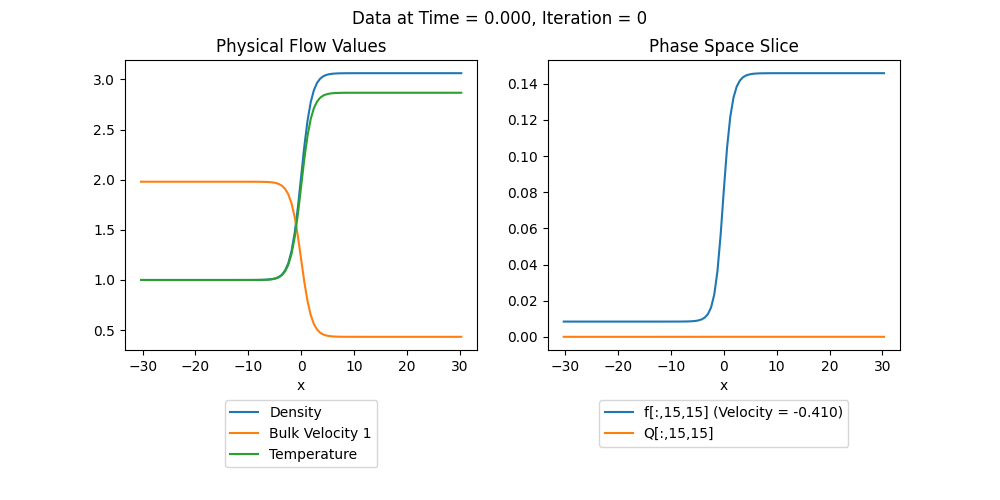
\includegraphics[width=\textwidth]{imgs/ts_output2/plots/plot0.png}
  \end{subfigure}
  \hfill
  \begin{subfigure}[b]{\textwidth}
  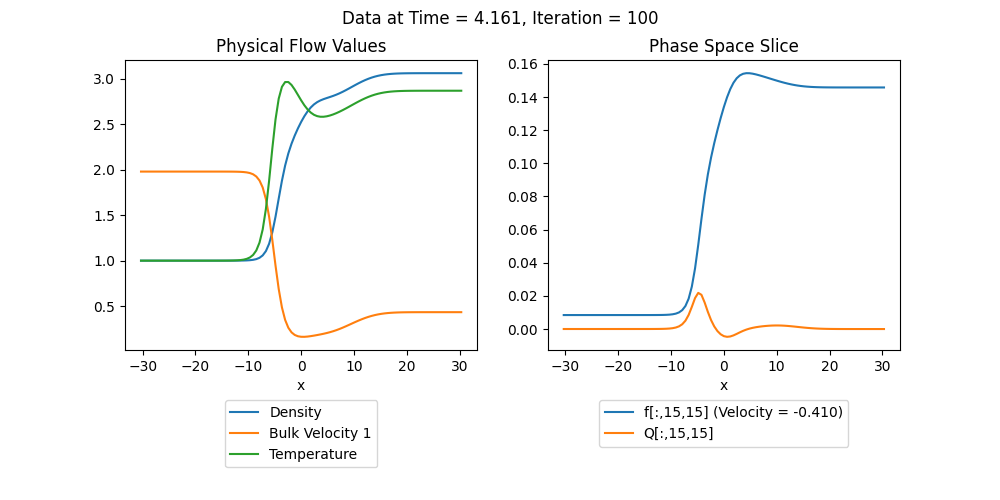
\includegraphics[width=\textwidth]{imgs/ts_output2/plots/plot100.png}
  \end{subfigure}
\end{figure}

\begin{figure}[H]
  \begin{subfigure}[b]{\textwidth}
    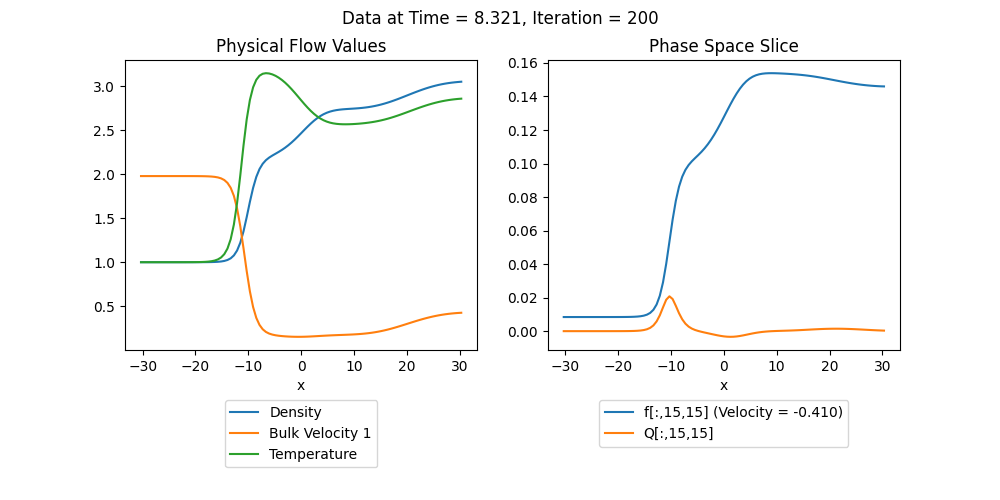
\includegraphics[width=\textwidth]{imgs/ts_output2/plots/plot200.png}
  \end{subfigure}
  \hfill
  \begin{subfigure}[b]{\textwidth}
    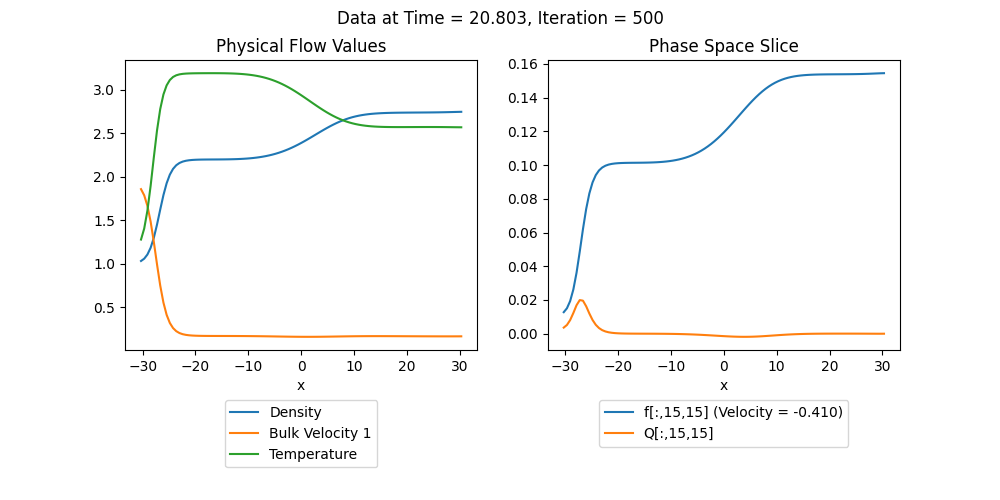
\includegraphics[width=\textwidth]{imgs/ts_output2/plots/plot500.png}
    \end{subfigure}
\end{figure}

\begin{figure}[H]
    \begin{subfigure}[b]{\textwidth}
    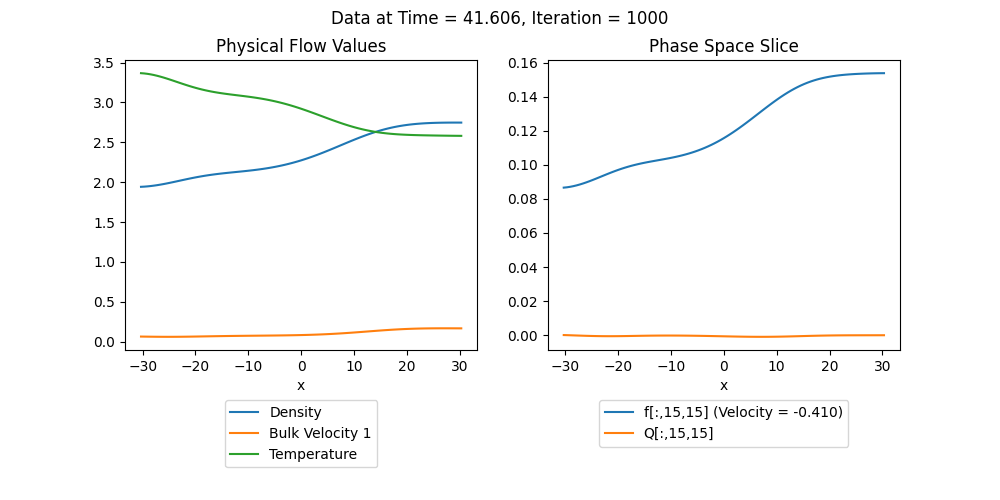
\includegraphics[width=\textwidth]{imgs/ts_output2/plots/plot1000.png}
    \end{subfigure}
    \hfill
    \begin{subfigure}[b]{\textwidth}
    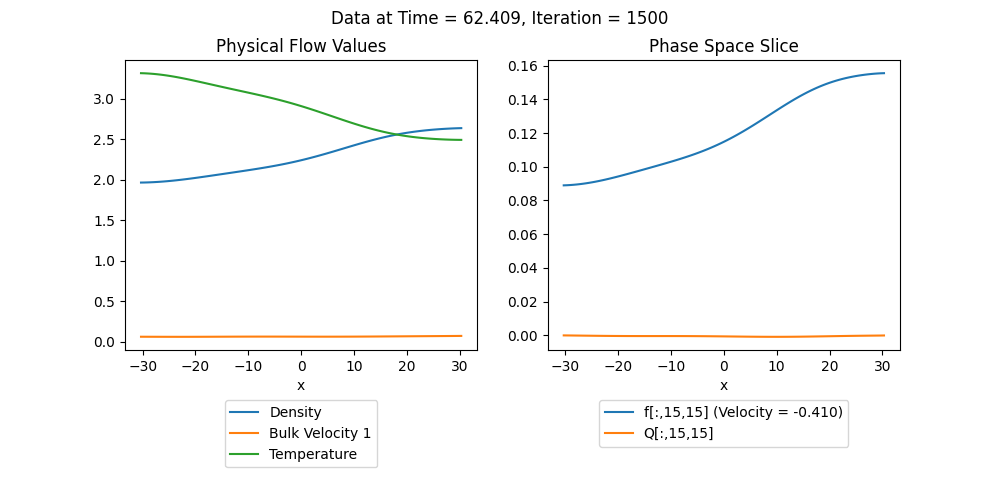
\includegraphics[width=\textwidth]{imgs/ts_output2/plots/plot1500.png}
    \end{subfigure}
\end{figure}
\subsubsection{Collision Kernel}
Here we display the phase space density function sliced at different values of $x$ alongside the two ways of computing the collision kernel. Note that the results of computing the collision kernel do not match. This implies that there is a difference between the theory and the implementation.
\begin{figure}[H]
  \begin{subfigure}[b]{\textwidth}
    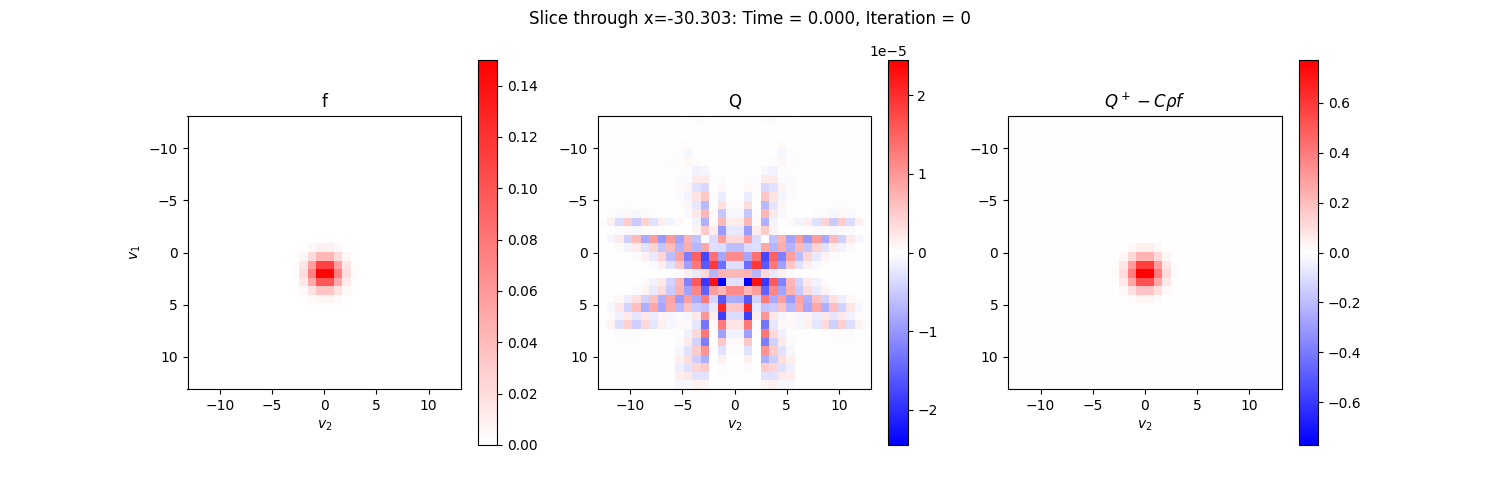
\includegraphics[width=\textwidth]{imgs/ts_output2/slice0/mat0.png}
  \end{subfigure}
  \hfill
  \begin{subfigure}[b]{\textwidth}
    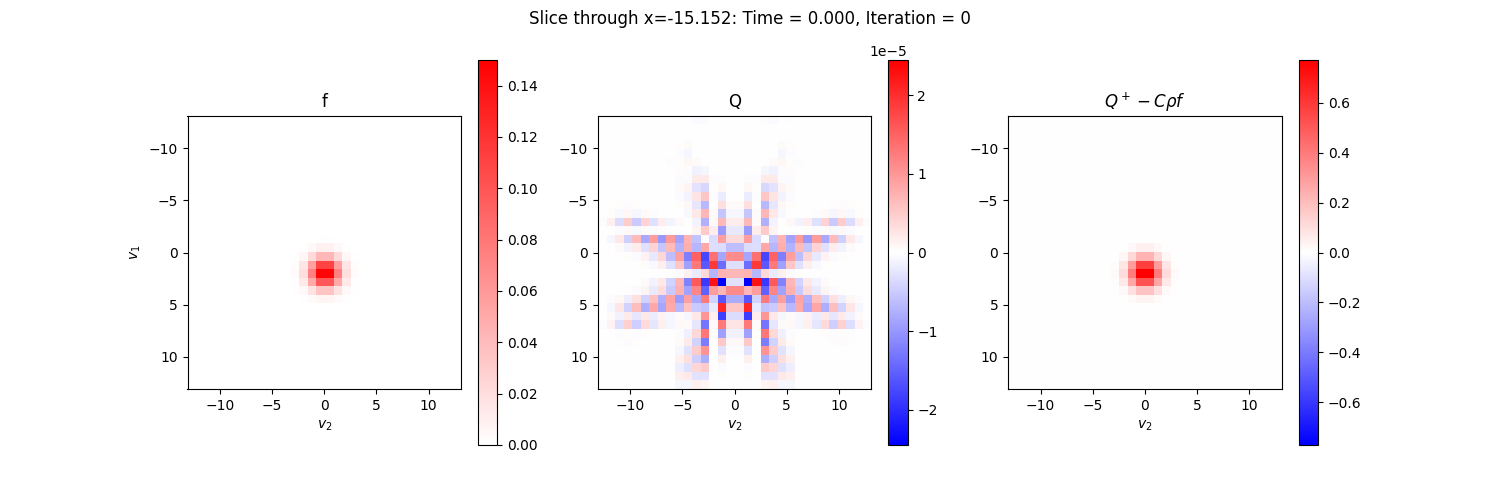
\includegraphics[width=\textwidth]{imgs/ts_output2/slice25/mat0.png}
  \end{subfigure}
  \hfill
  \begin{subfigure}[b]{\textwidth}
    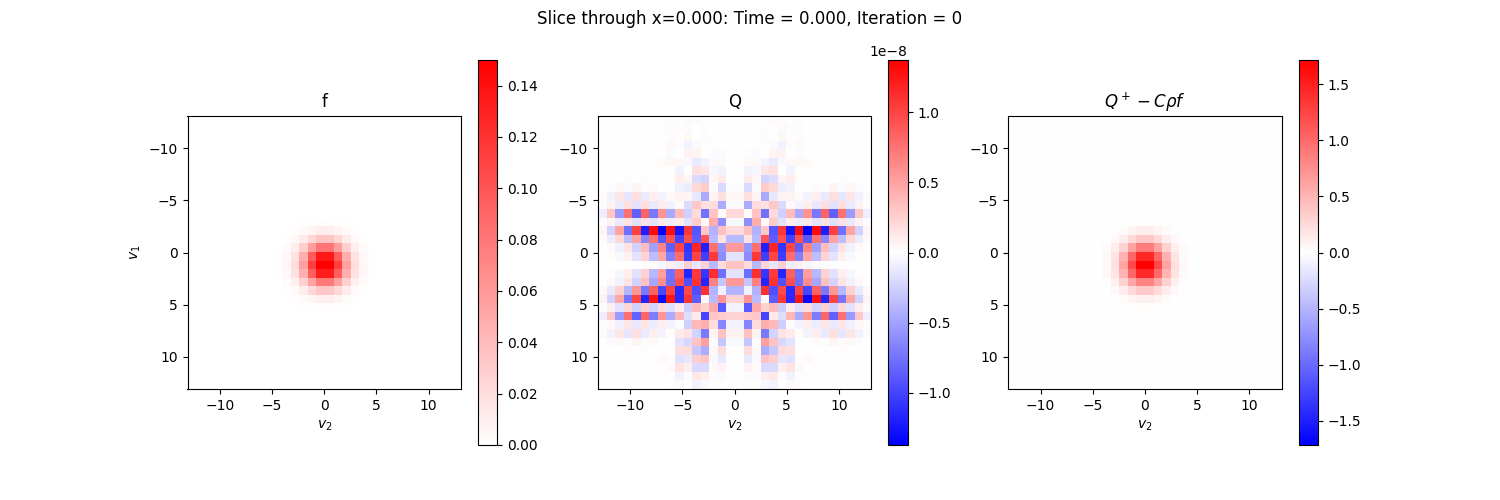
\includegraphics[width=\textwidth]{imgs/ts_output2/slice50/mat0.png}
  \end{subfigure}
  \hfill
  \begin{subfigure}[b]{\textwidth}
    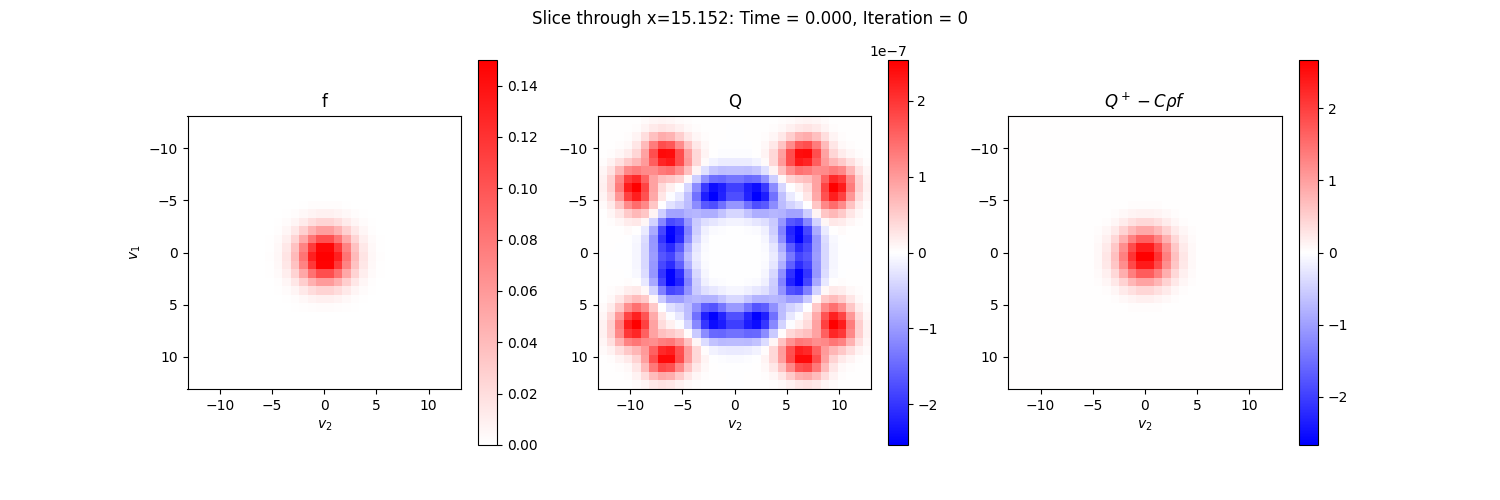
\includegraphics[width=\textwidth]{imgs/ts_output2/slice75/mat0.png}
  \end{subfigure}
\end{figure}

\begin{figure}[H]
  \begin{subfigure}[b]{\textwidth}
    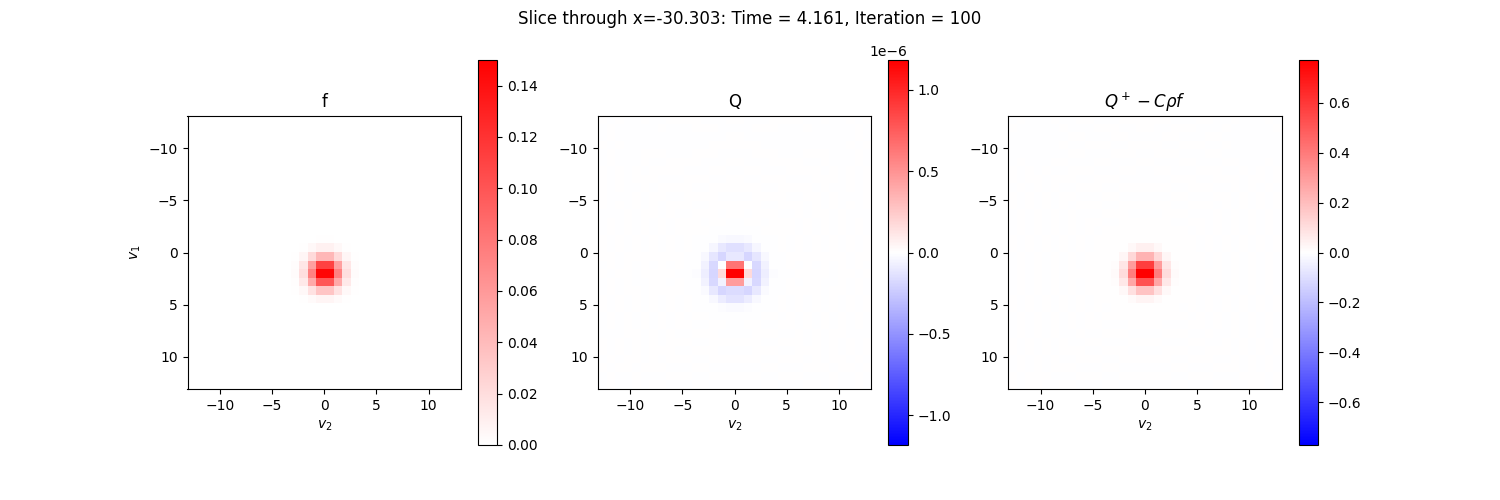
\includegraphics[width=\textwidth]{imgs/ts_output2/slice0/mat100.png}
  \end{subfigure}
  \hfill
  \begin{subfigure}[b]{\textwidth}
    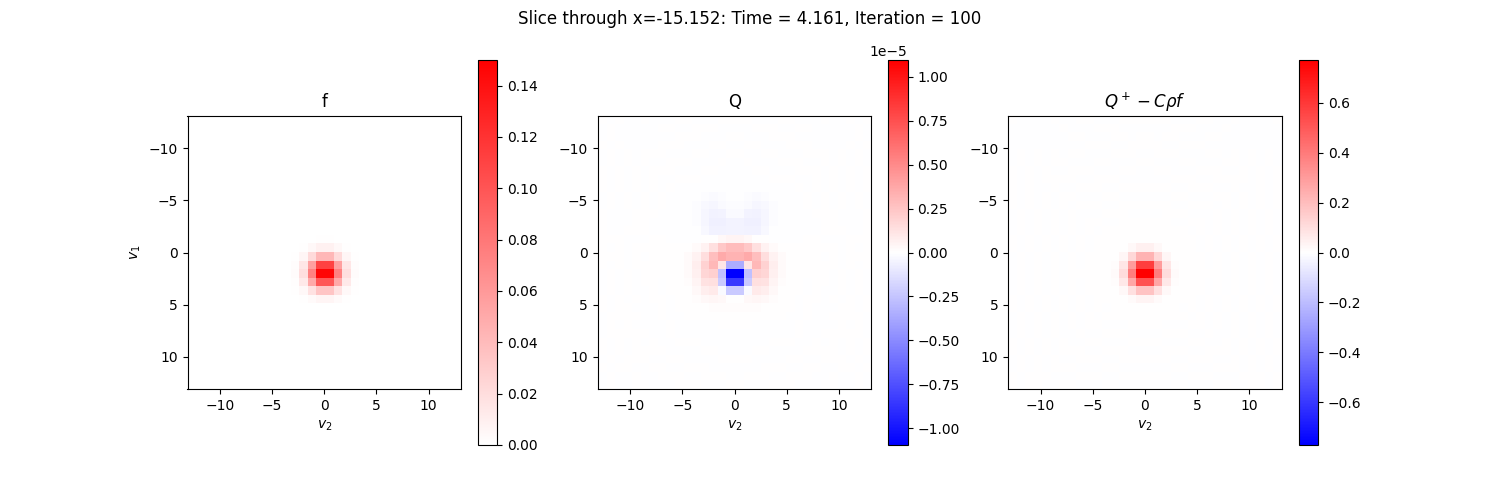
\includegraphics[width=\textwidth]{imgs/ts_output2/slice25/mat100.png}
  \end{subfigure}
  \hfill
  \begin{subfigure}[b]{\textwidth}
    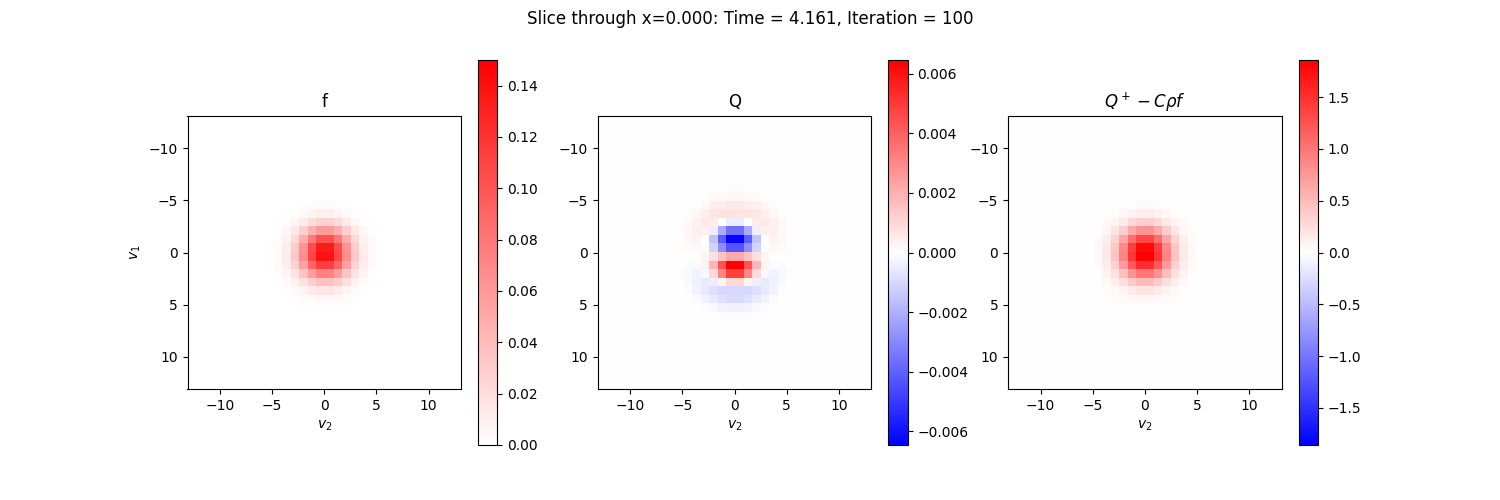
\includegraphics[width=\textwidth]{imgs/ts_output2/slice50/mat100.png}
  \end{subfigure}
  \hfill
  \begin{subfigure}[b]{\textwidth}
    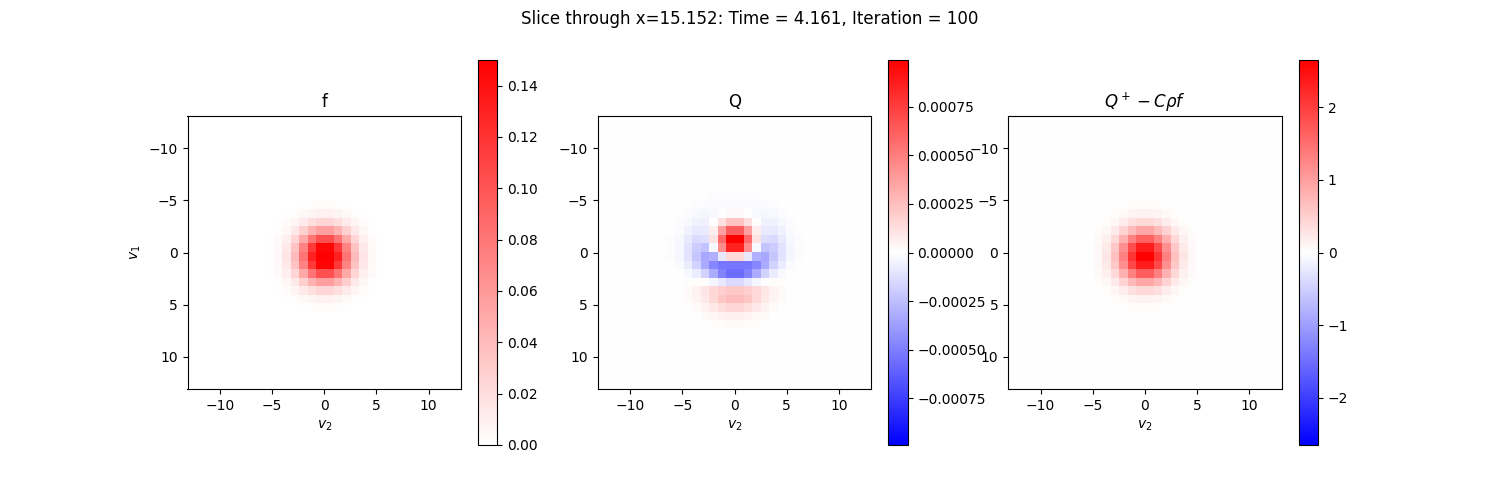
\includegraphics[width=\textwidth]{imgs/ts_output2/slice75/mat100.png}
  \end{subfigure}
\end{figure}

\begin{figure}[H]
  \begin{subfigure}[b]{\textwidth}
    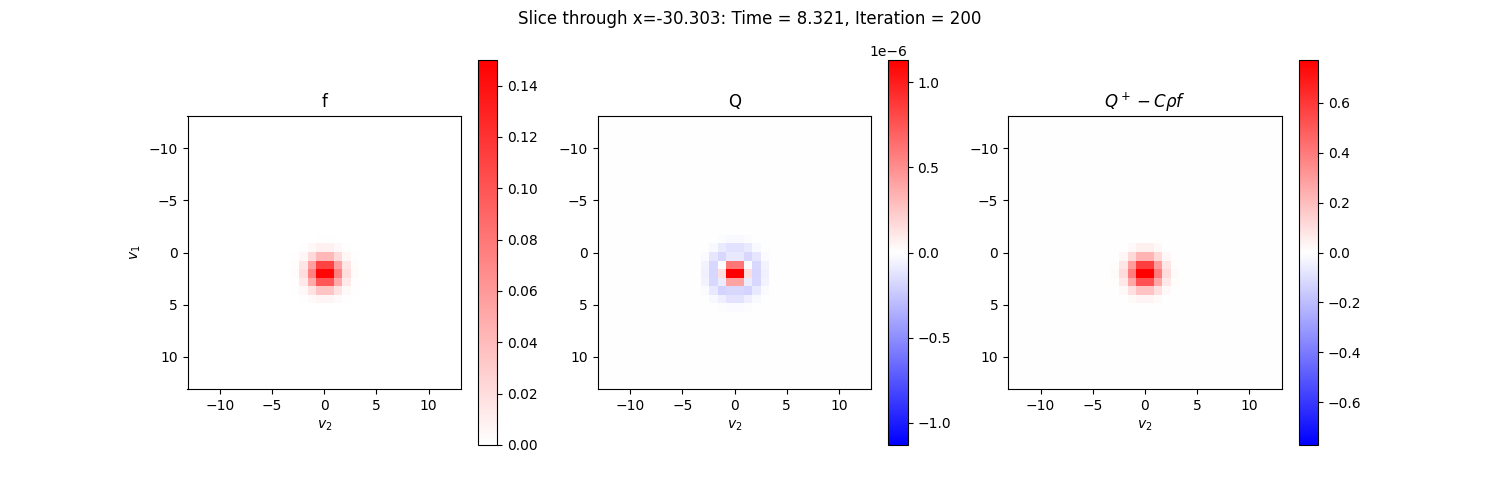
\includegraphics[width=\textwidth]{imgs/ts_output2/slice0/mat200.png}
  \end{subfigure}
  \hfill
  \begin{subfigure}[b]{\textwidth}
    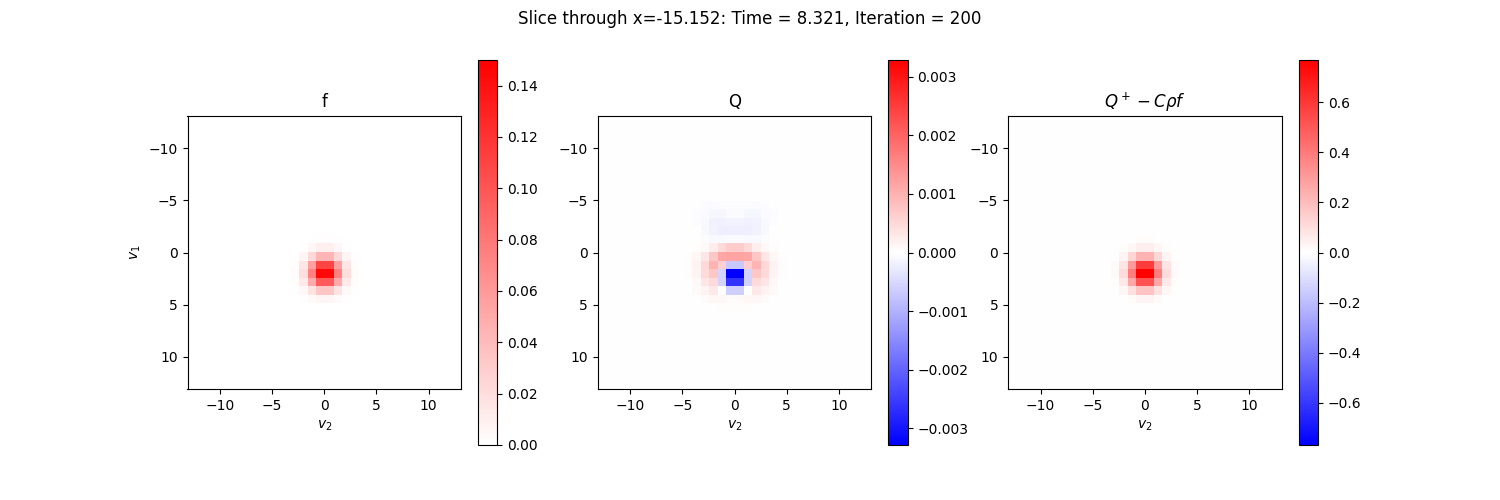
\includegraphics[width=\textwidth]{imgs/ts_output2/slice25/mat200.png}
  \end{subfigure}
  \hfill
  \begin{subfigure}[b]{\textwidth}
    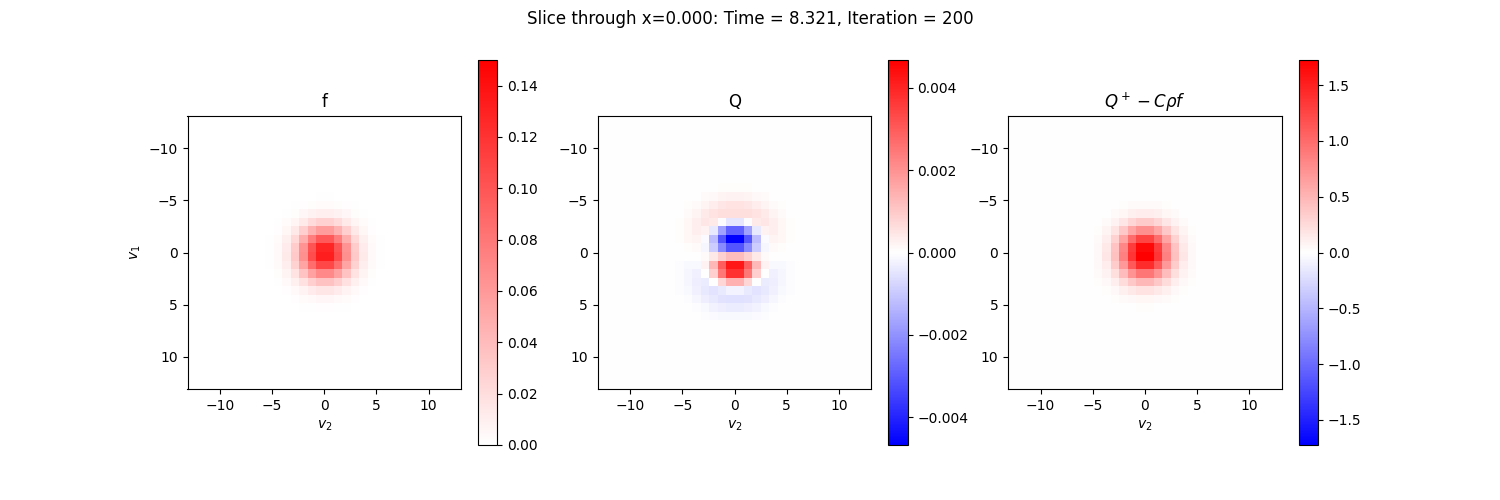
\includegraphics[width=\textwidth]{imgs/ts_output2/slice50/mat200.png}
  \end{subfigure}
  \hfill
  \begin{subfigure}[b]{\textwidth}
    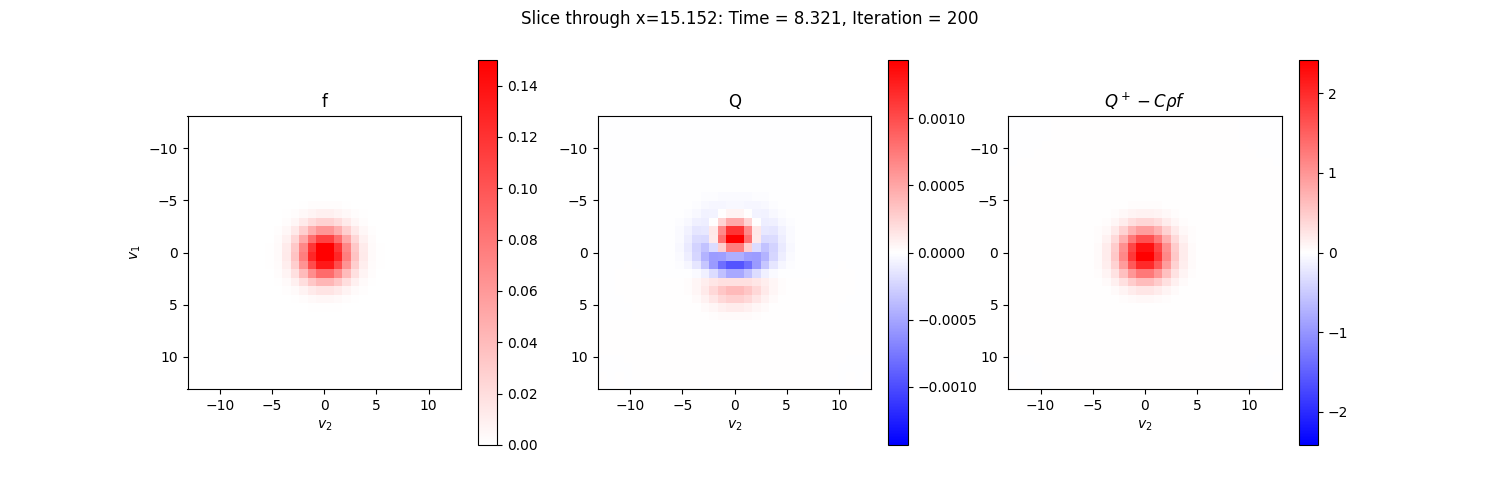
\includegraphics[width=\textwidth]{imgs/ts_output2/slice75/mat200.png}
  \end{subfigure}
\end{figure}

\begin{figure}[H]
  \begin{subfigure}[b]{\textwidth}
    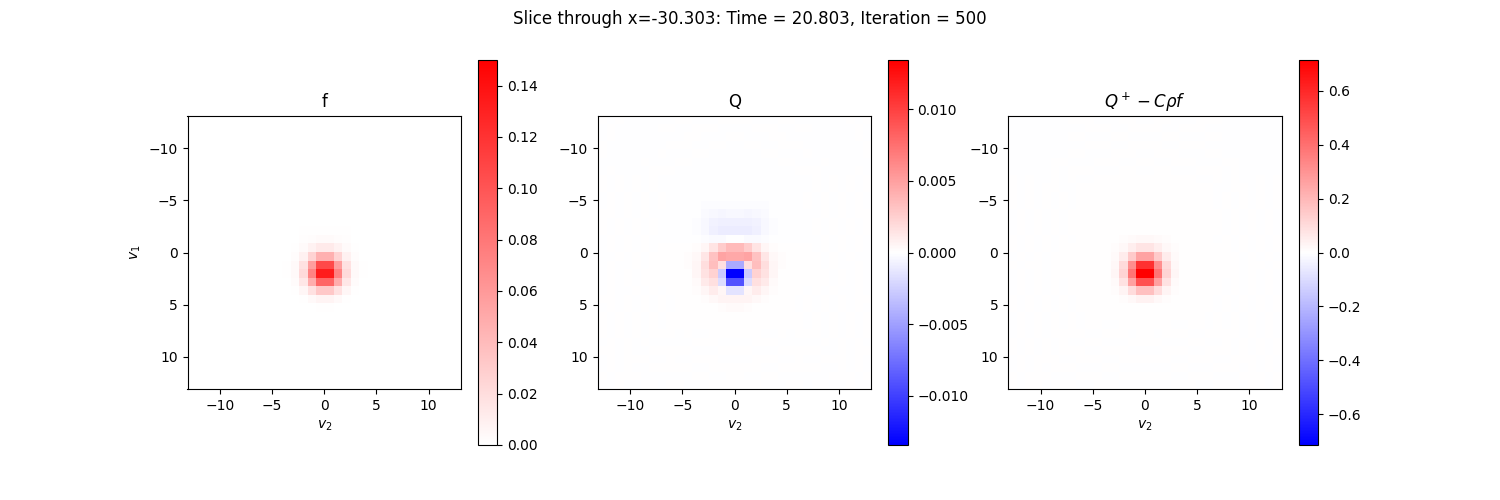
\includegraphics[width=\textwidth]{imgs/ts_output2/slice0/mat500.png}
  \end{subfigure}
  \hfill
  \begin{subfigure}[b]{\textwidth}
    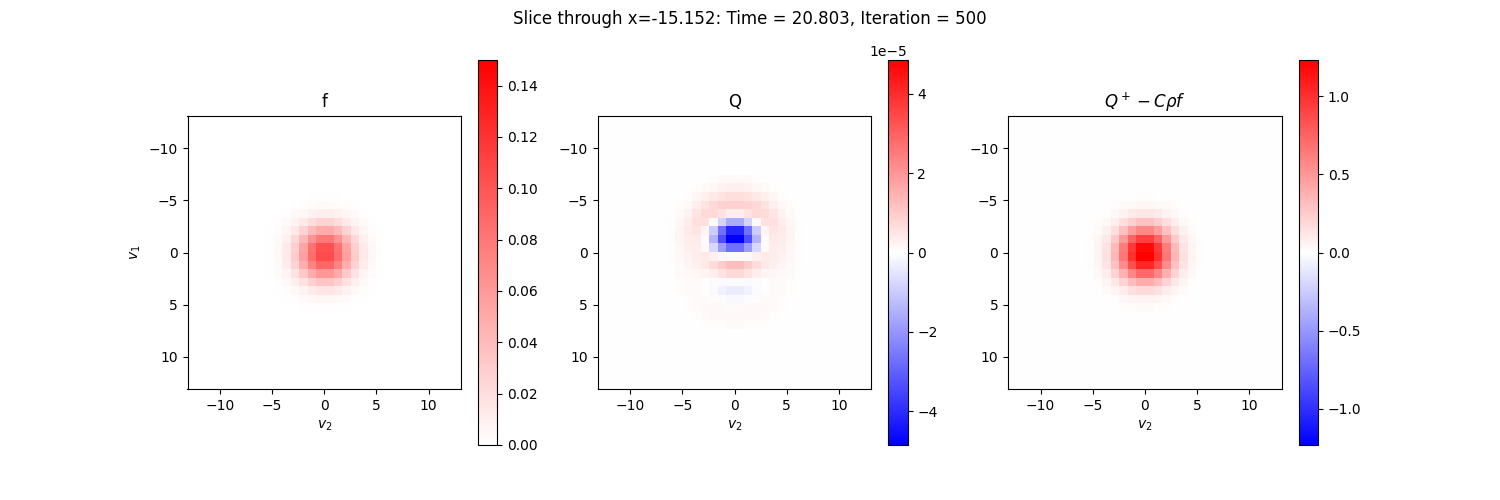
\includegraphics[width=\textwidth]{imgs/ts_output2/slice25/mat500.png}
  \end{subfigure}
  \hfill
  \begin{subfigure}[b]{\textwidth}
    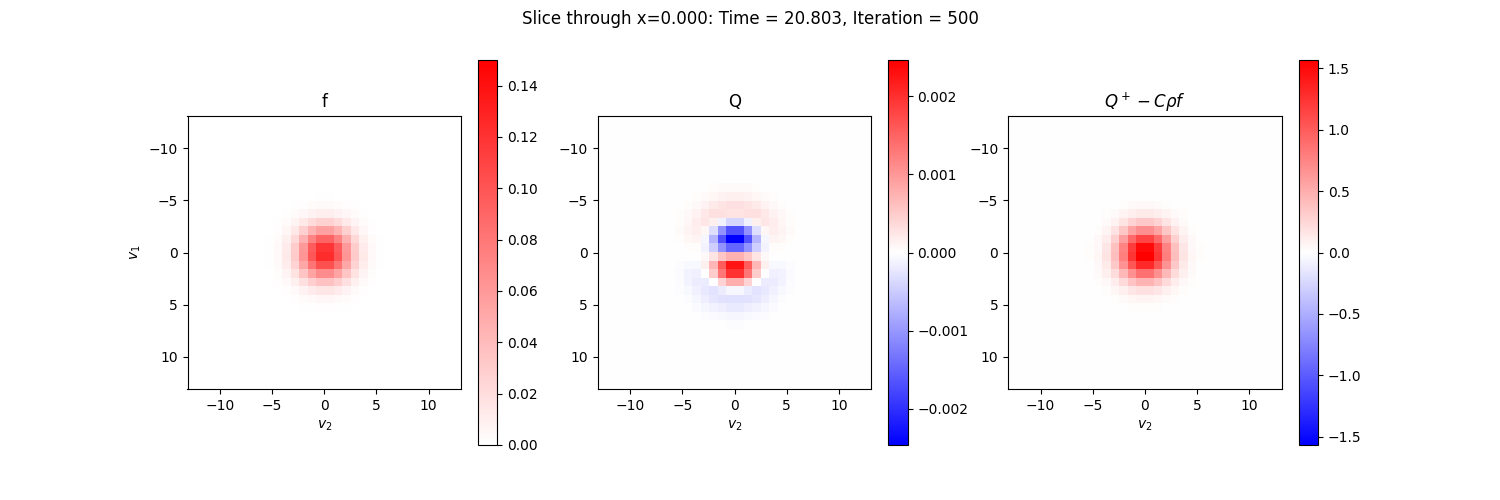
\includegraphics[width=\textwidth]{imgs/ts_output2/slice50/mat500.png}
  \end{subfigure}
  \hfill
  \begin{subfigure}[b]{\textwidth}
    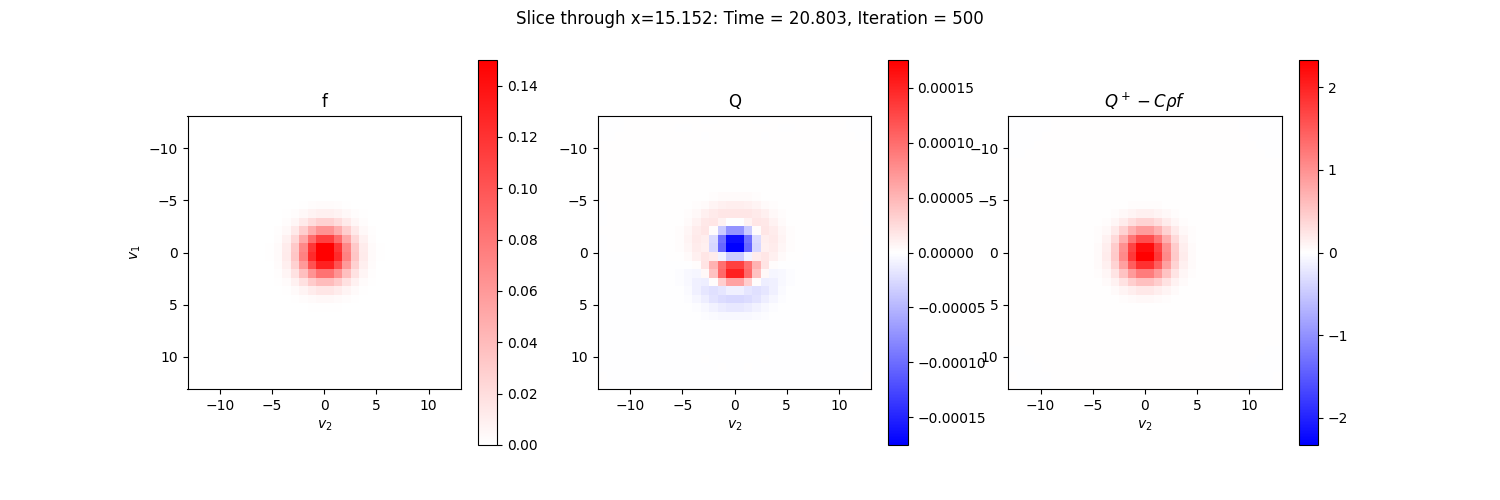
\includegraphics[width=\textwidth]{imgs/ts_output2/slice75/mat500.png}
  \end{subfigure}
\end{figure}

\begin{figure}[H]
  \begin{subfigure}[b]{\textwidth}
    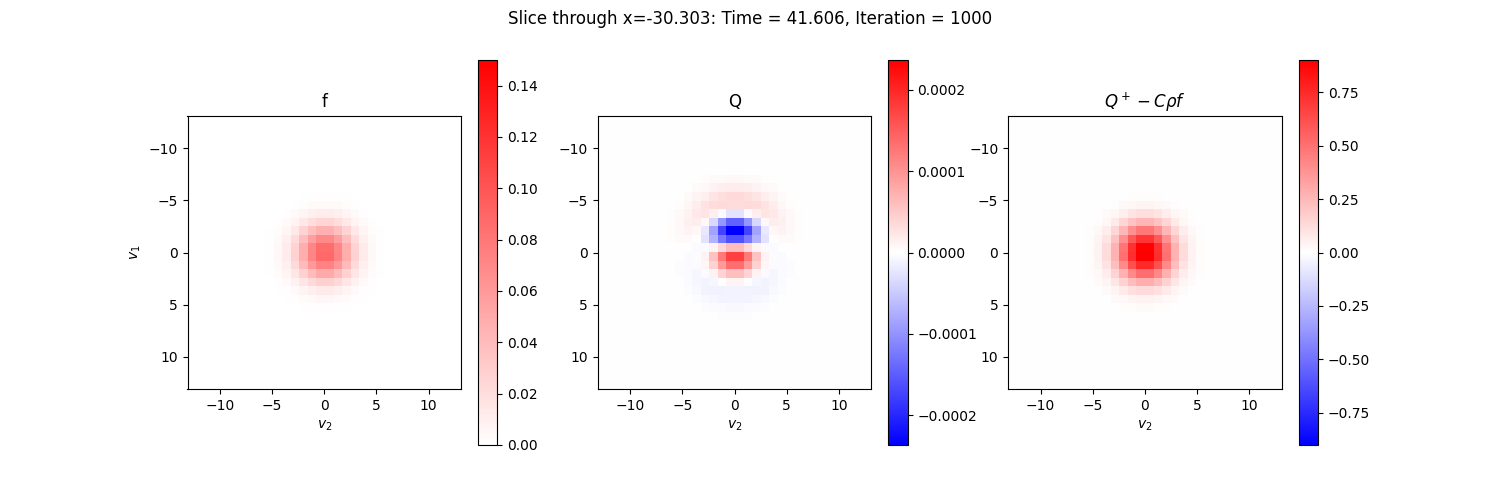
\includegraphics[width=\textwidth]{imgs/ts_output2/slice0/mat1000.png}
  \end{subfigure}
  \hfill
  \begin{subfigure}[b]{\textwidth}
    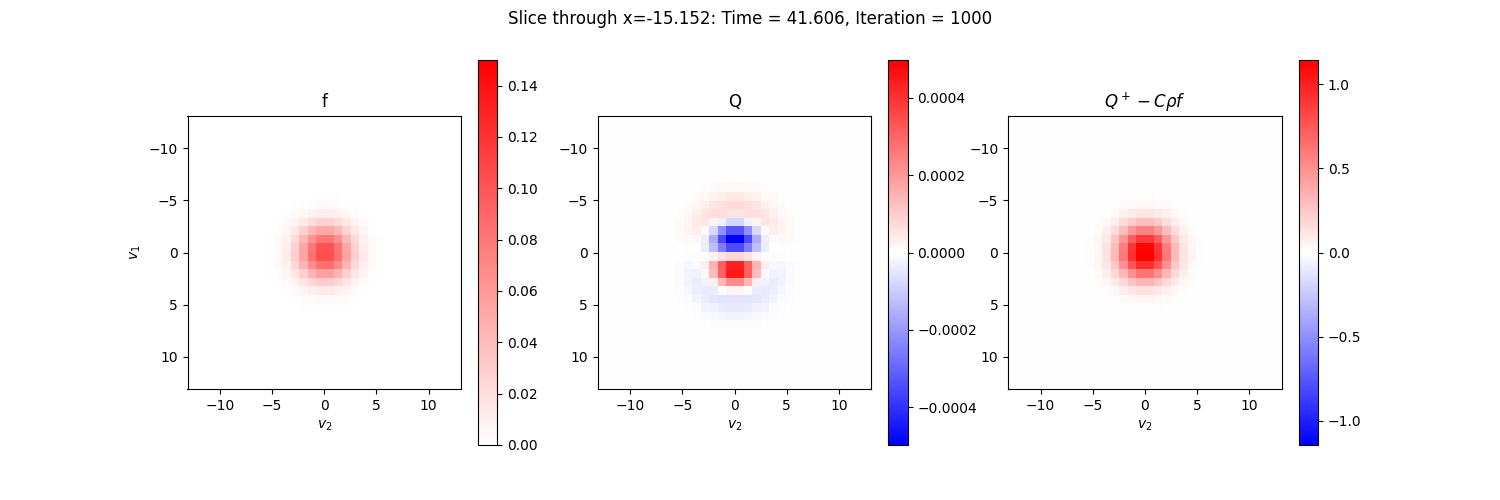
\includegraphics[width=\textwidth]{imgs/ts_output2/slice25/mat1000.png}
  \end{subfigure}
  \hfill
  \begin{subfigure}[b]{\textwidth}
    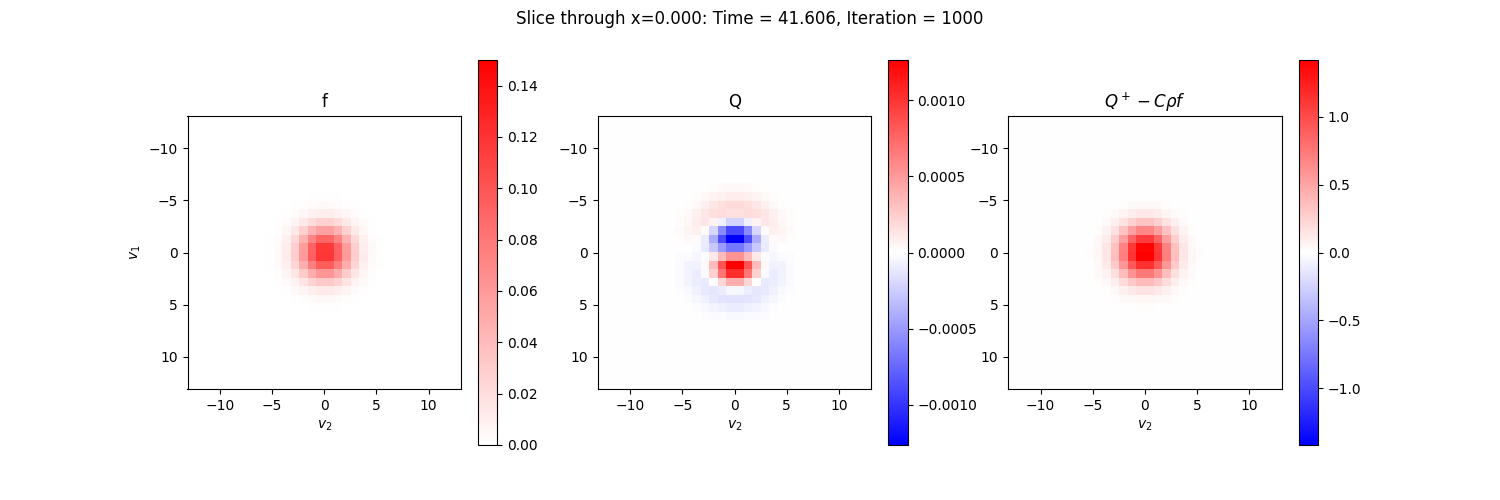
\includegraphics[width=\textwidth]{imgs/ts_output2/slice50/mat1000.png}
  \end{subfigure}
  \hfill
  \begin{subfigure}[b]{\textwidth}
    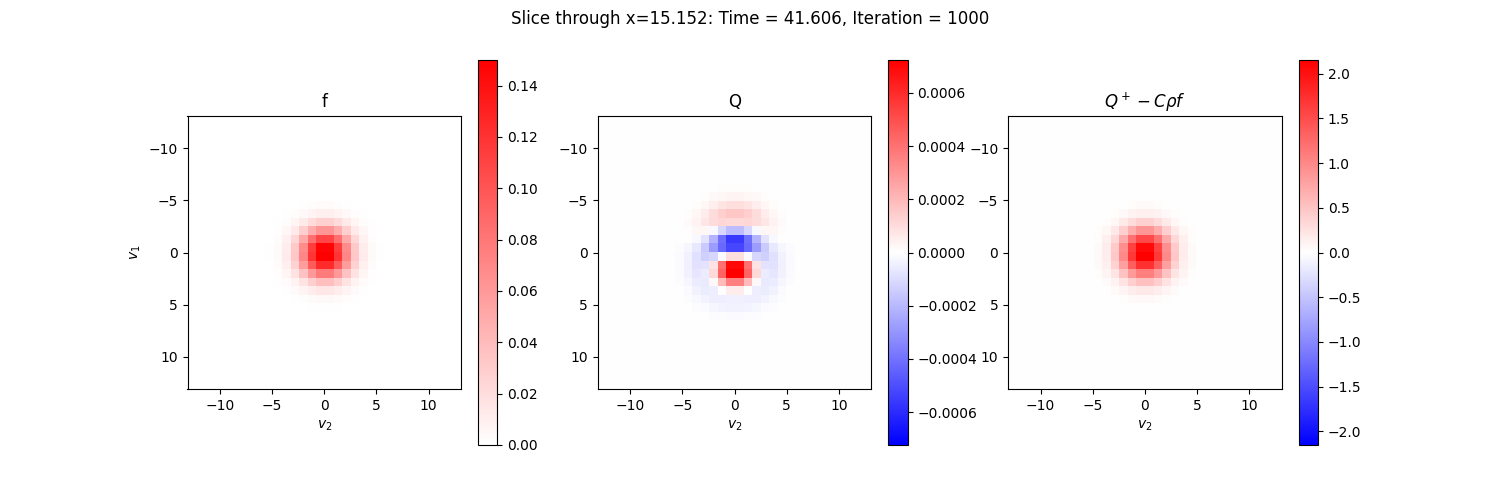
\includegraphics[width=\textwidth]{imgs/ts_output2/slice75/mat1000.png}
  \end{subfigure}
\end{figure}

\begin{figure}[H]
  \begin{subfigure}[b]{\textwidth}
    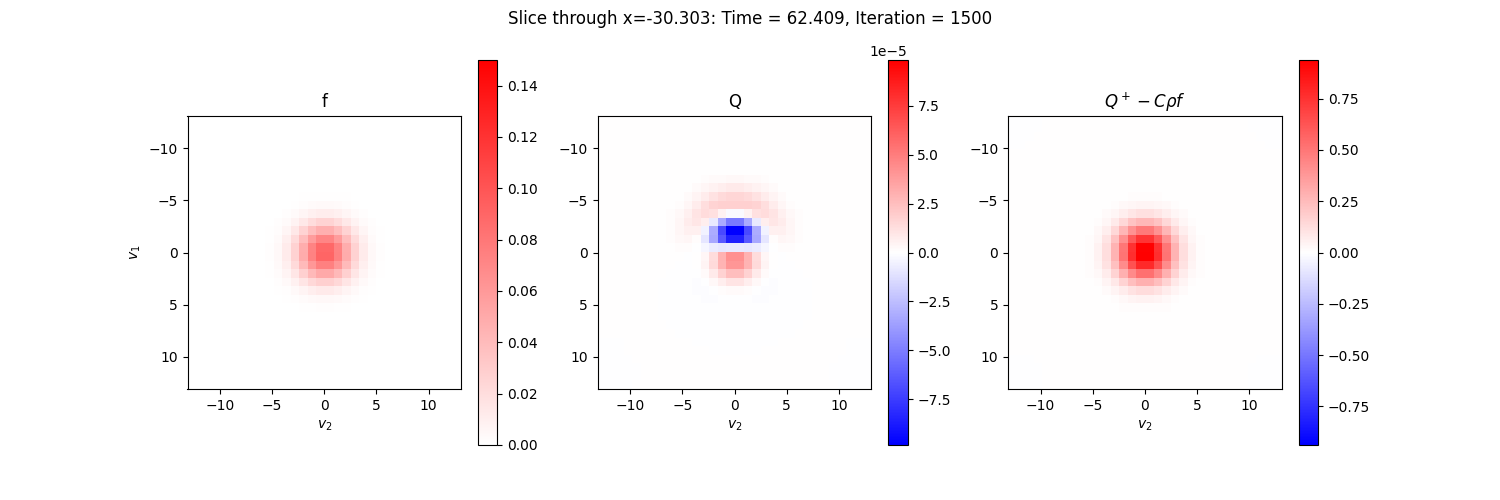
\includegraphics[width=\textwidth]{imgs/ts_output2/slice0/mat1500.png}
  \end{subfigure}
  \hfill
  \begin{subfigure}[b]{\textwidth}
    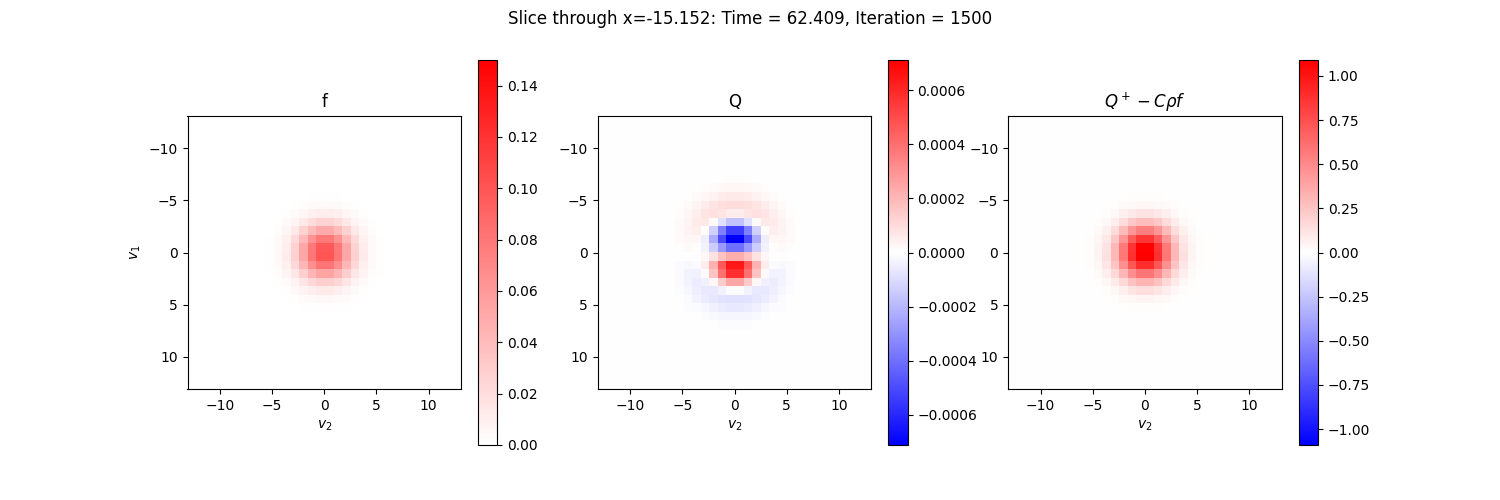
\includegraphics[width=\textwidth]{imgs/ts_output2/slice25/mat1500.png}
  \end{subfigure}
  \hfill
  \begin{subfigure}[b]{\textwidth}
    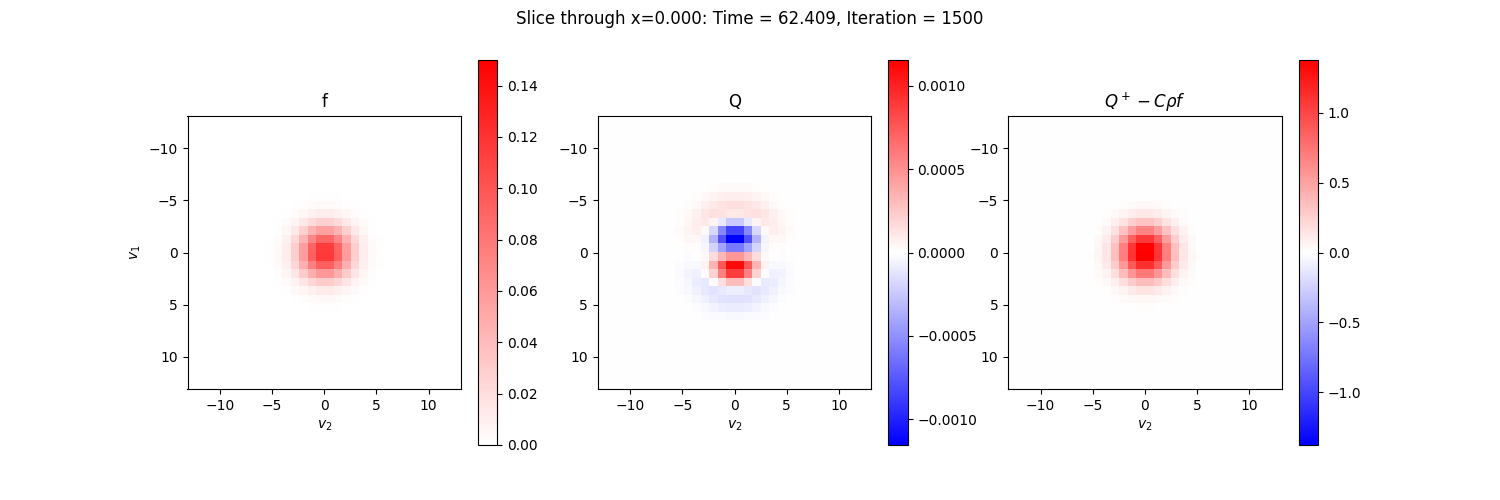
\includegraphics[width=\textwidth]{imgs/ts_output2/slice50/mat1500.png}
  \end{subfigure}
  \hfill
  \begin{subfigure}[b]{\textwidth}
    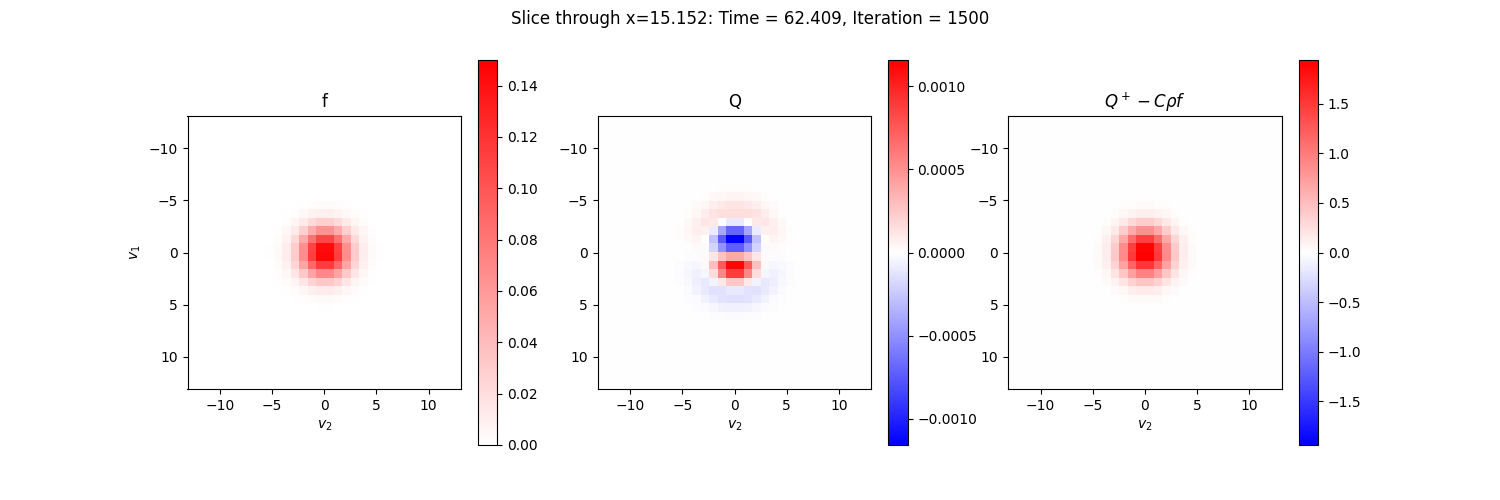
\includegraphics[width=\textwidth]{imgs/ts_output2/slice75/mat1500.png}
  \end{subfigure}
\end{figure}

\subsection{Lax-Friedrichs Fast Sweeping Results}
\subsubsection{Pressure, Bulk Velocity, and Temperature Results}
\begin{figure}[H]
  \begin{subfigure}[b]{\textwidth}
  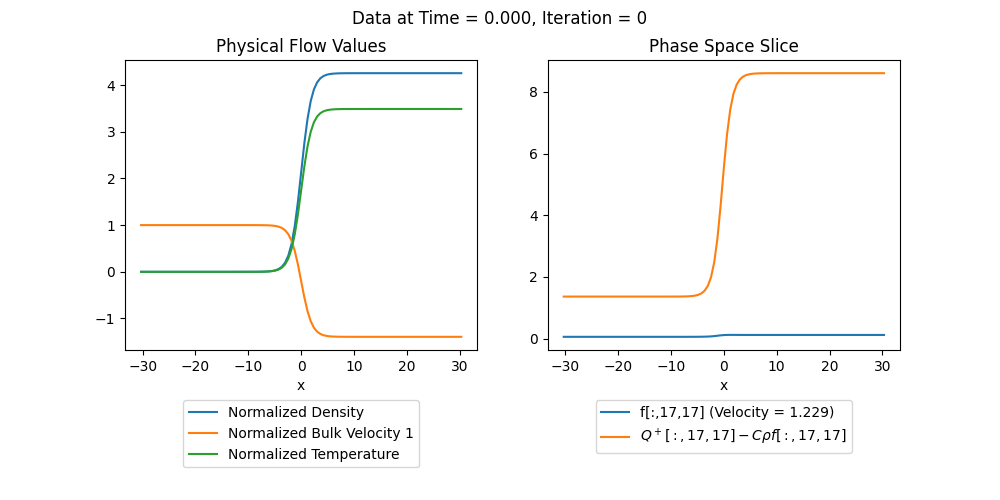
\includegraphics[width=\textwidth]{imgs/lf_output2/plots/plot0.png}
  \end{subfigure}
  \hfill
  \begin{subfigure}[b]{\textwidth}
  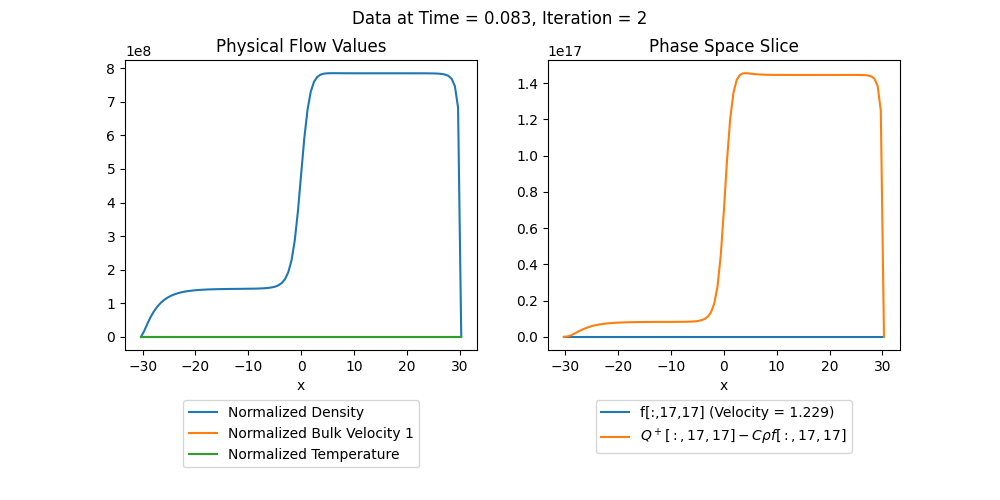
\includegraphics[width=\textwidth]{imgs/lf_output2/plots/plot2.png}
  \end{subfigure}
\end{figure}

\begin{figure}[H]
  \begin{subfigure}[b]{\textwidth}
    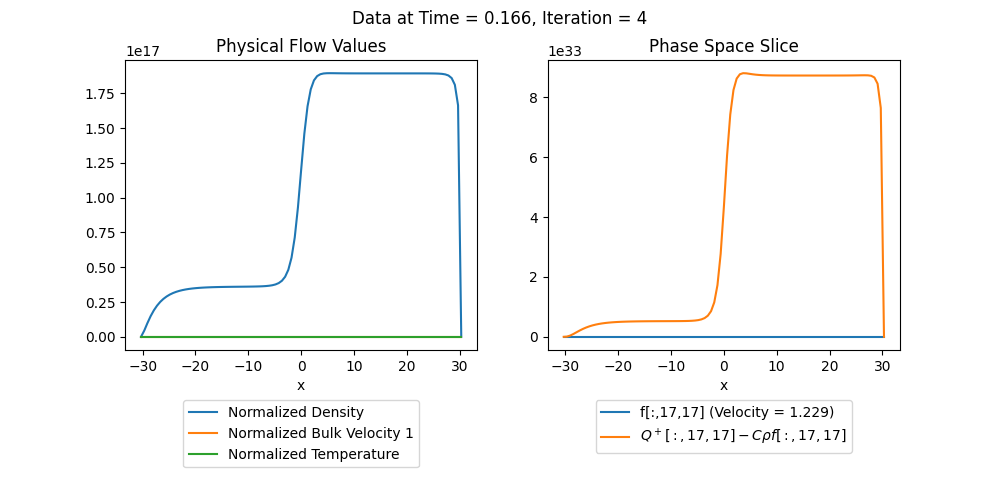
\includegraphics[width=\textwidth]{imgs/lf_output2/plots/plot4.png}
  \end{subfigure}
  \hfill
  \begin{subfigure}[b]{\textwidth}
    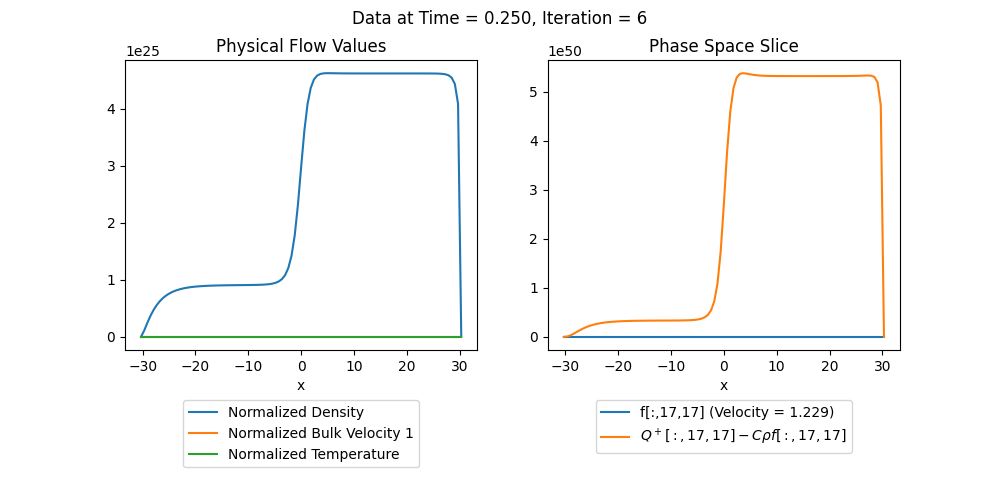
\includegraphics[width=\textwidth]{imgs/lf_output2/plots/plot6.png}
    \end{subfigure}
\end{figure}

\begin{figure}[H]
    \begin{subfigure}[b]{\textwidth}
    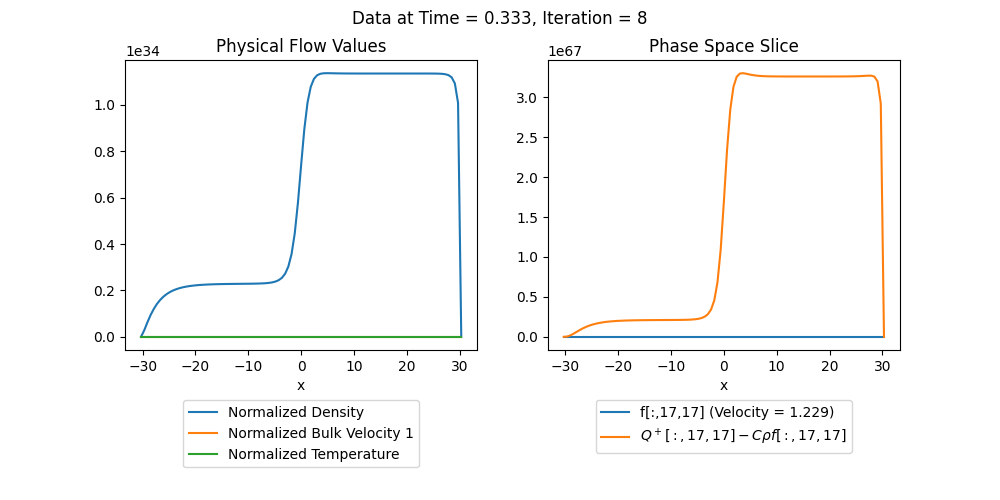
\includegraphics[width=\textwidth]{imgs/lf_output2/plots/plot8.png}
    \end{subfigure}
    \hfill
    \begin{subfigure}[b]{\textwidth}
    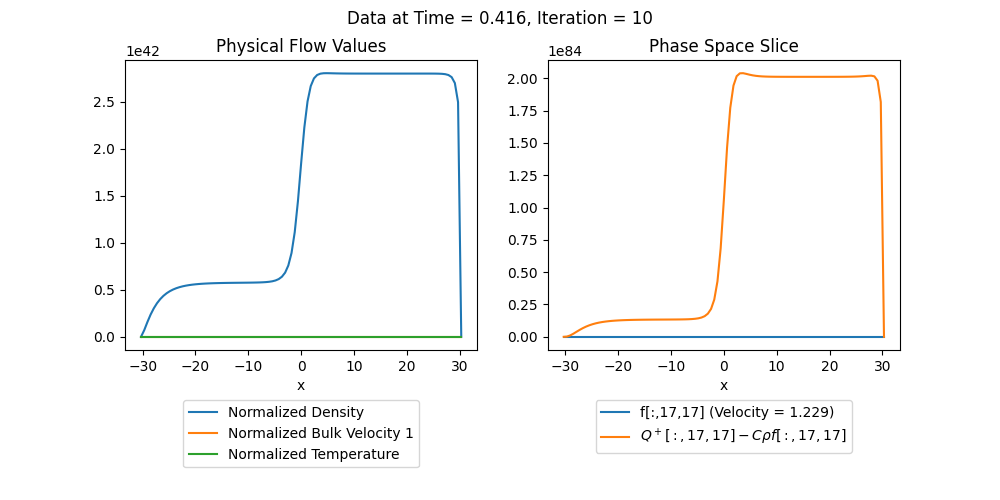
\includegraphics[width=\textwidth]{imgs/lf_output2/plots/plot10.png}
    \end{subfigure}
\end{figure}
\subsubsection{Collision Kernel}
Here we display the phase space density function sliced at different values of $x$ alongside the two ways of computing the collision kernel. Note that the results of computing the collision kernel do not match. This implies that there is a difference between the theory and the implementation.
\begin{figure}[H]
  \begin{subfigure}[b]{\textwidth}
    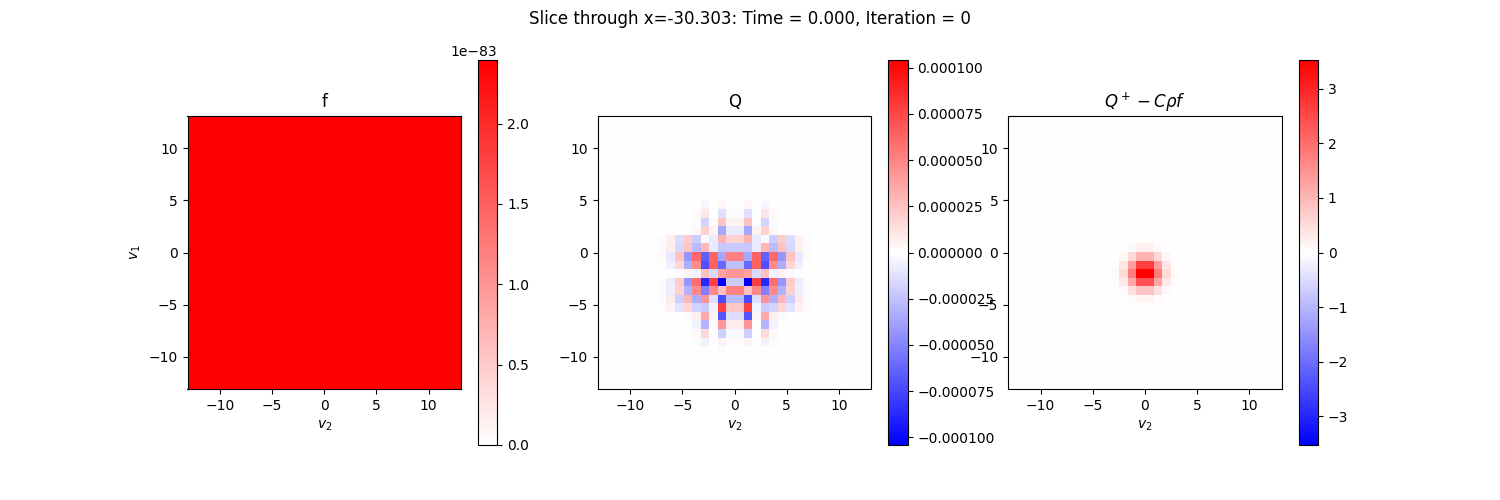
\includegraphics[width=\textwidth]{imgs/lf_output2/slice0/mat0.png}
  \end{subfigure}
  \hfill
  \begin{subfigure}[b]{\textwidth}
    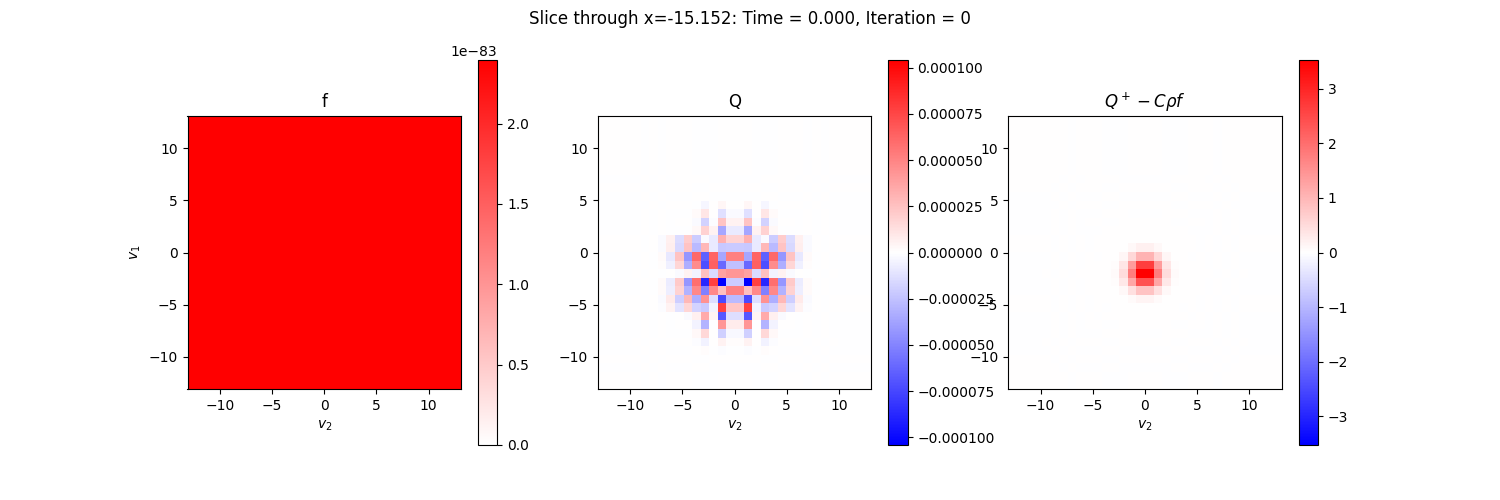
\includegraphics[width=\textwidth]{imgs/lf_output2/slice25/mat0.png}
  \end{subfigure}
  \hfill
  \begin{subfigure}[b]{\textwidth}
    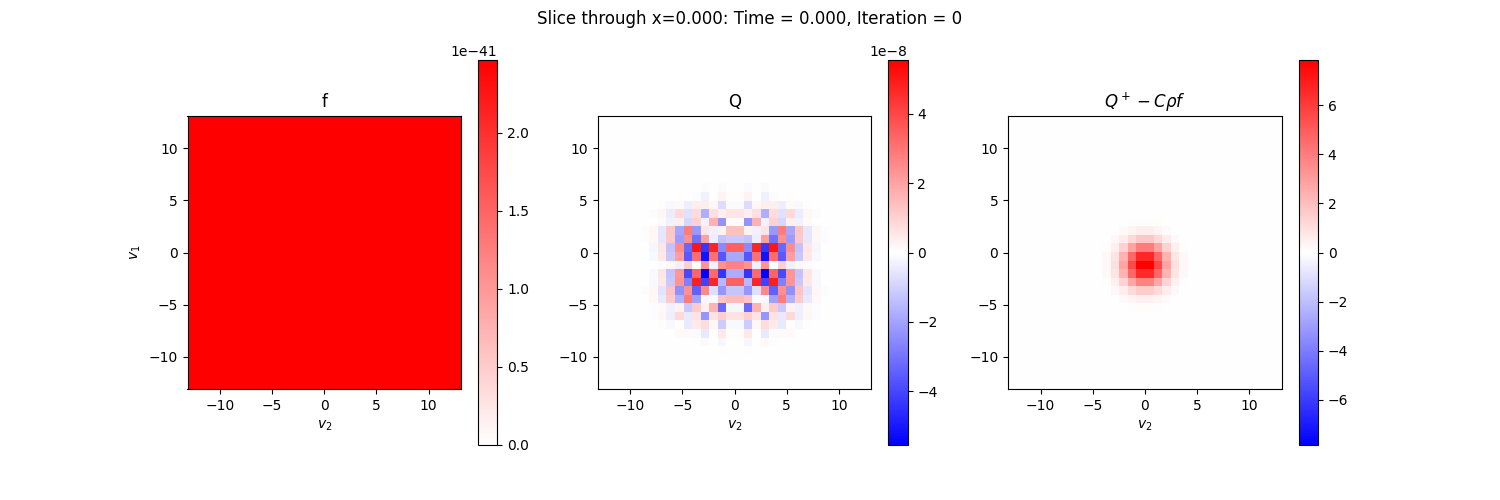
\includegraphics[width=\textwidth]{imgs/lf_output2/slice50/mat0.png}
  \end{subfigure}
  \hfill
  \begin{subfigure}[b]{\textwidth}
    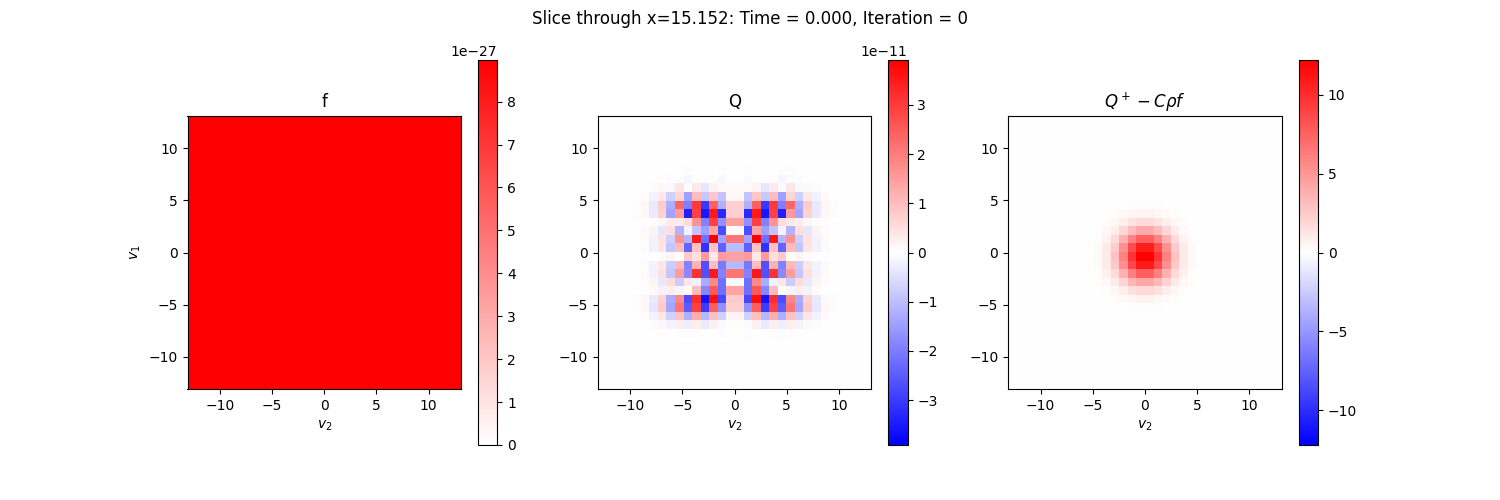
\includegraphics[width=\textwidth]{imgs/lf_output2/slice75/mat0.png}
  \end{subfigure}
\end{figure}

\begin{figure}[H]
  \begin{subfigure}[b]{\textwidth}
    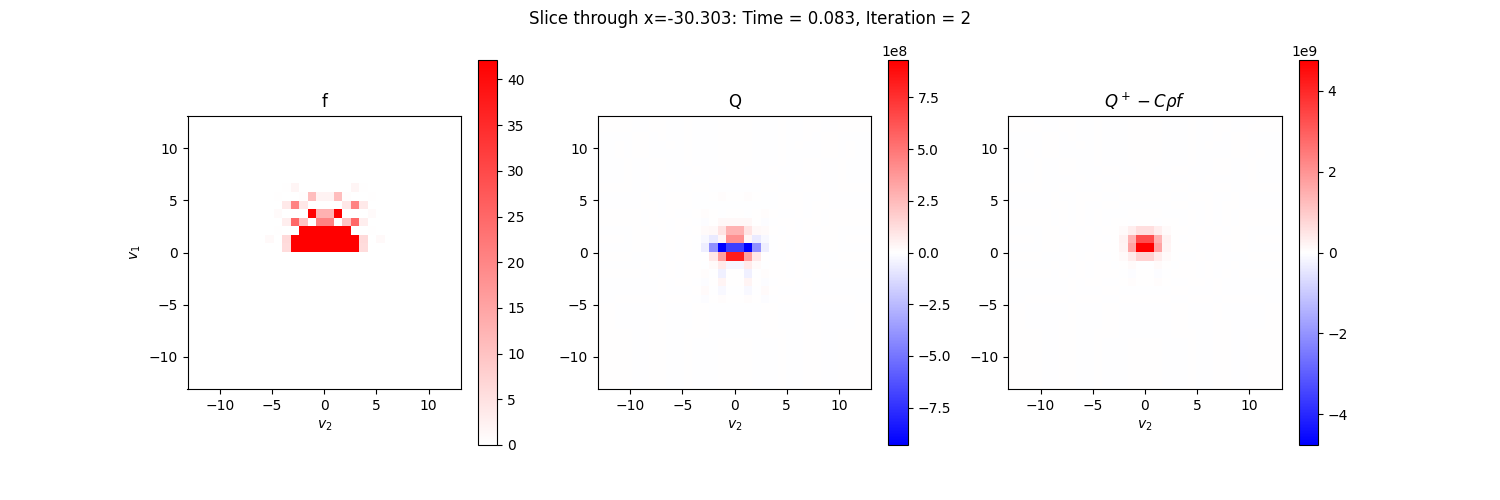
\includegraphics[width=\textwidth]{imgs/lf_output2/slice0/mat2.png}
  \end{subfigure}
  \hfill
  \begin{subfigure}[b]{\textwidth}
    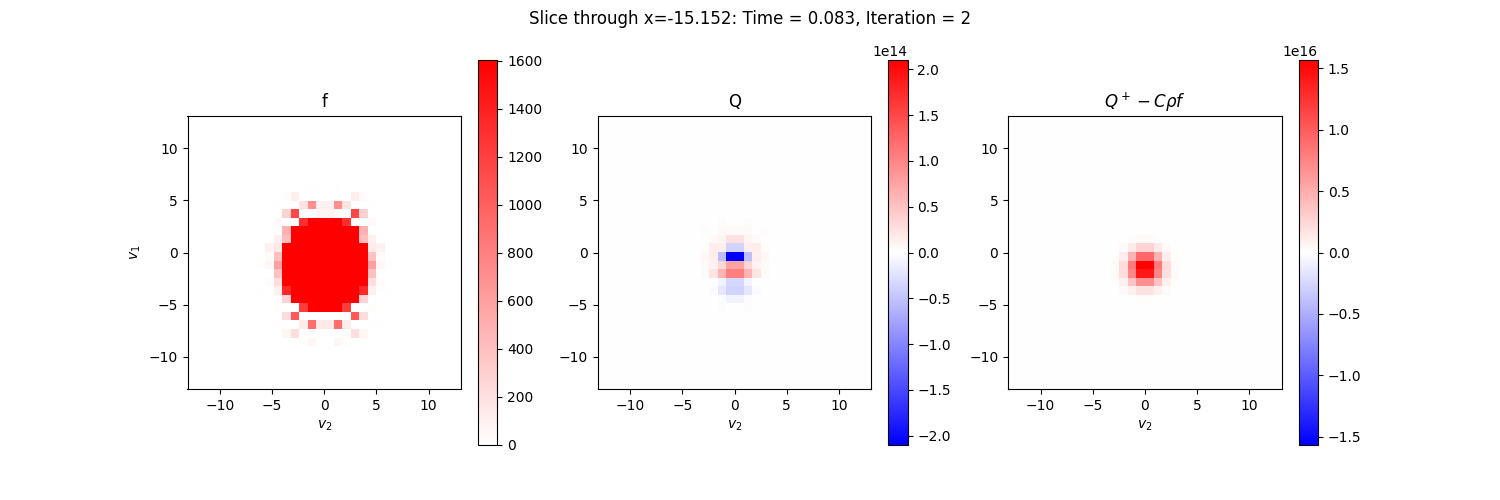
\includegraphics[width=\textwidth]{imgs/lf_output2/slice25/mat2.png}
  \end{subfigure}
  \hfill
  \begin{subfigure}[b]{\textwidth}
    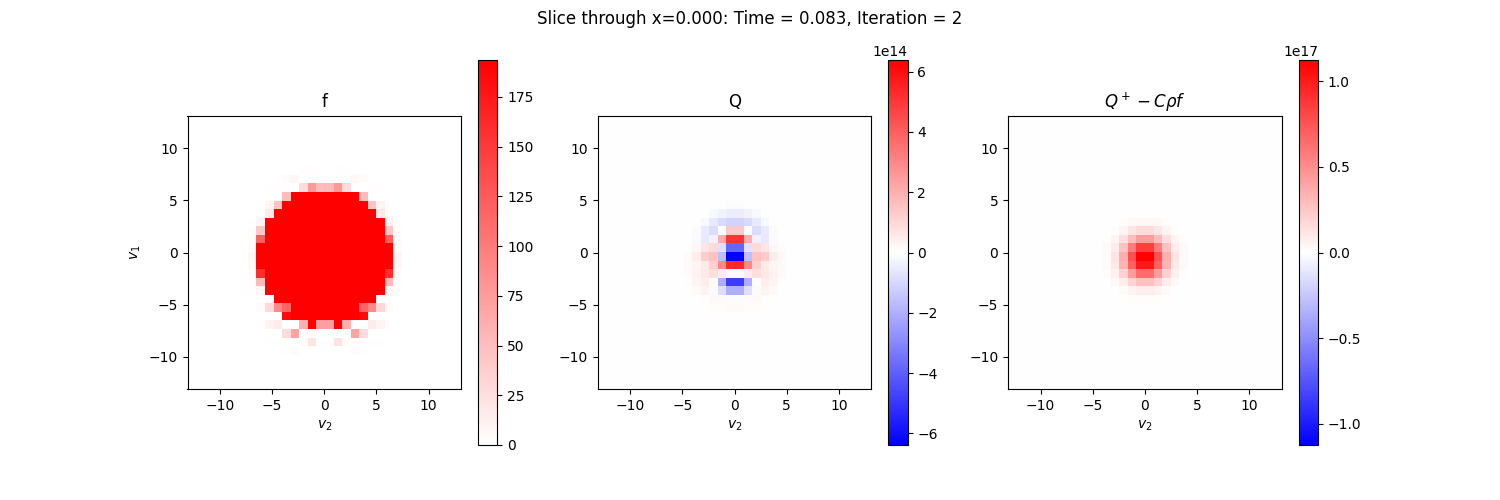
\includegraphics[width=\textwidth]{imgs/lf_output2/slice50/mat2.png}
  \end{subfigure}
  \hfill
  \begin{subfigure}[b]{\textwidth}
    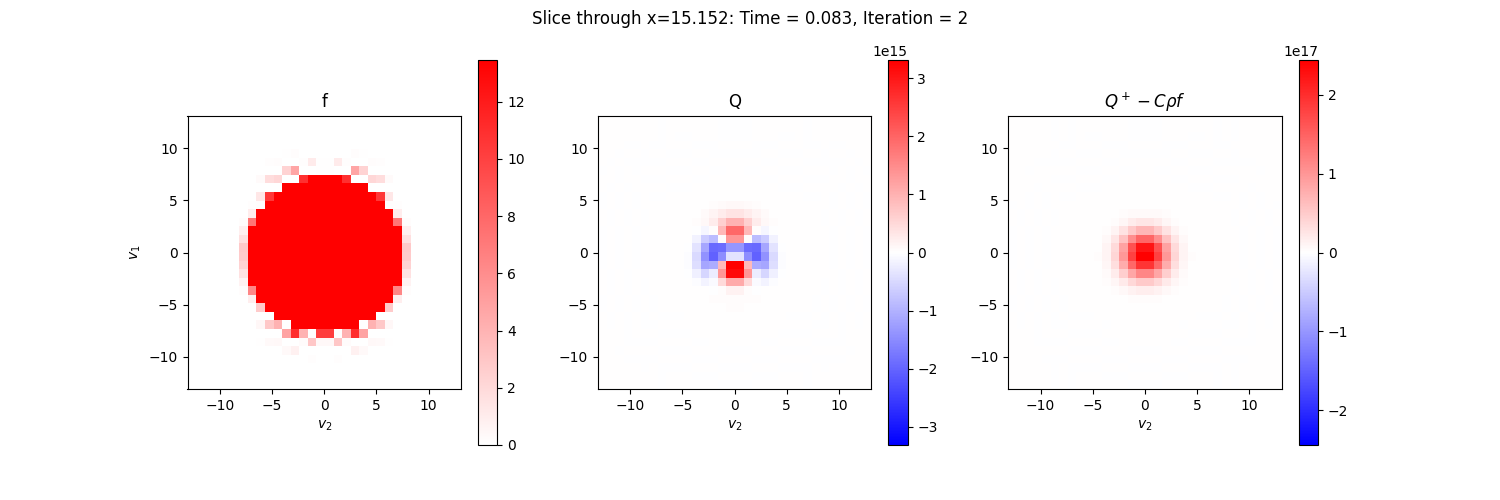
\includegraphics[width=\textwidth]{imgs/lf_output2/slice75/mat2.png}
  \end{subfigure}
\end{figure}

\begin{figure}[H]
  \begin{subfigure}[b]{\textwidth}
    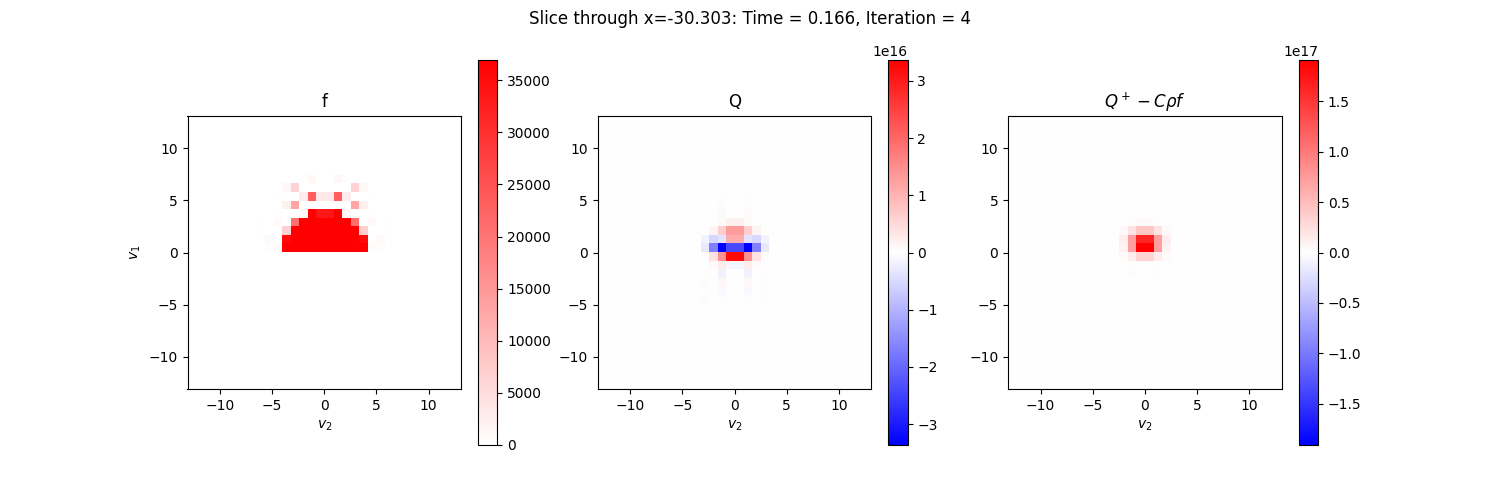
\includegraphics[width=\textwidth]{imgs/lf_output2/slice0/mat4.png}
  \end{subfigure}
  \hfill
  \begin{subfigure}[b]{\textwidth}
    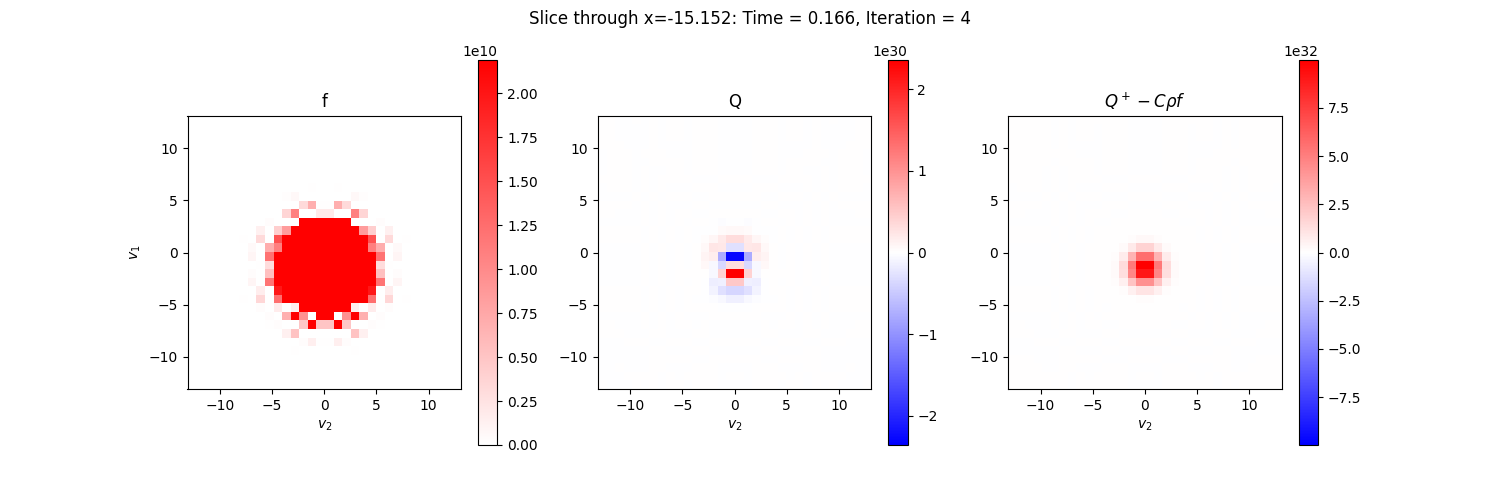
\includegraphics[width=\textwidth]{imgs/lf_output2/slice25/mat4.png}
  \end{subfigure}
  \hfill
  \begin{subfigure}[b]{\textwidth}
    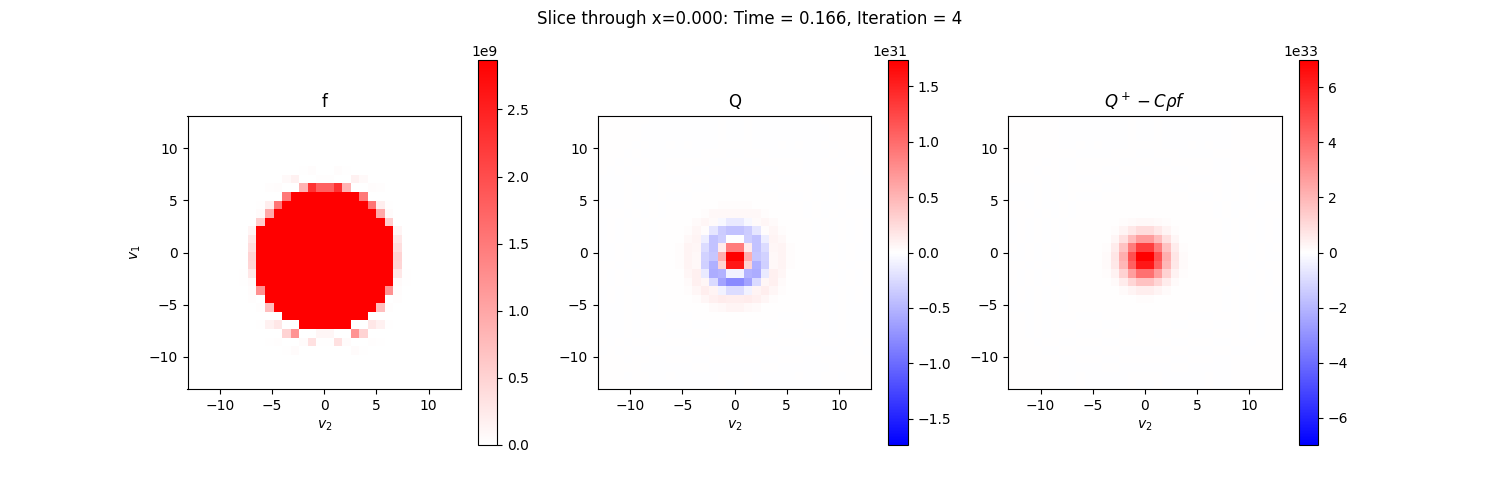
\includegraphics[width=\textwidth]{imgs/lf_output2/slice50/mat4.png}
  \end{subfigure}
  \hfill
  \begin{subfigure}[b]{\textwidth}
    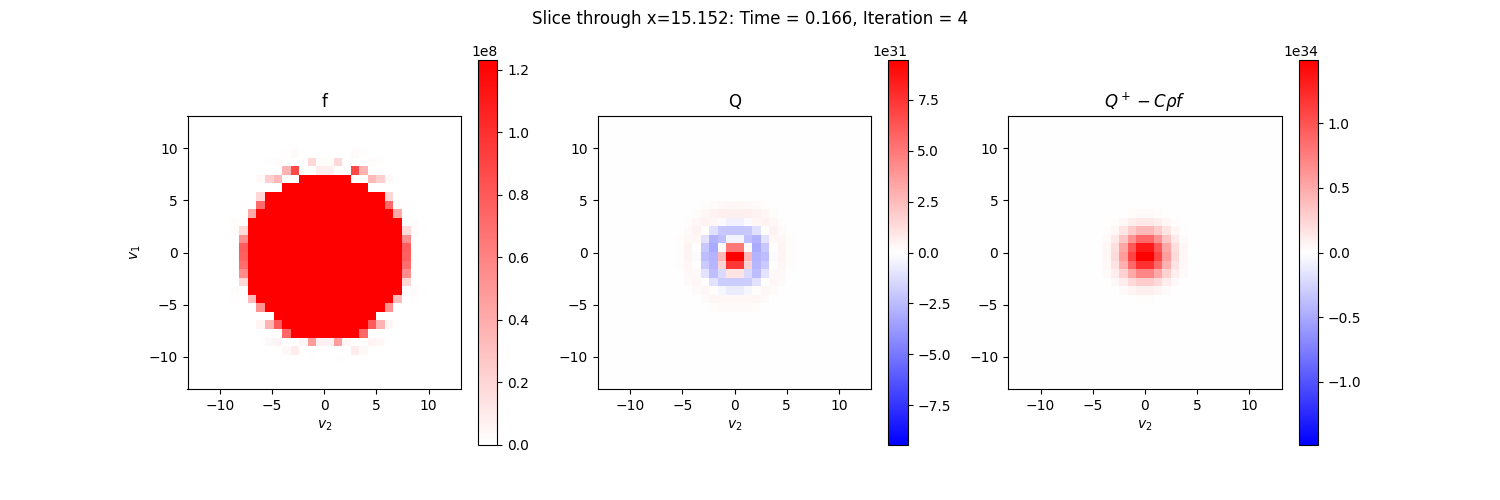
\includegraphics[width=\textwidth]{imgs/lf_output2/slice75/mat4.png}
  \end{subfigure}
\end{figure}

\begin{figure}[H]
  \begin{subfigure}[b]{\textwidth}
    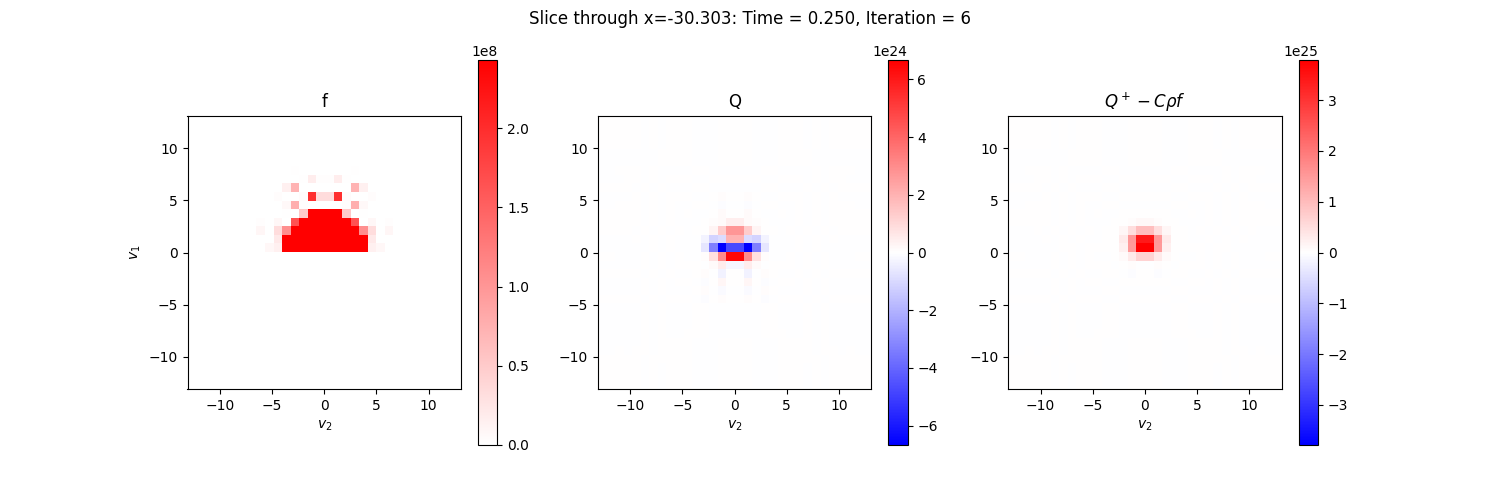
\includegraphics[width=\textwidth]{imgs/lf_output2/slice0/mat6.png}
  \end{subfigure}
  \hfill
  \begin{subfigure}[b]{\textwidth}
    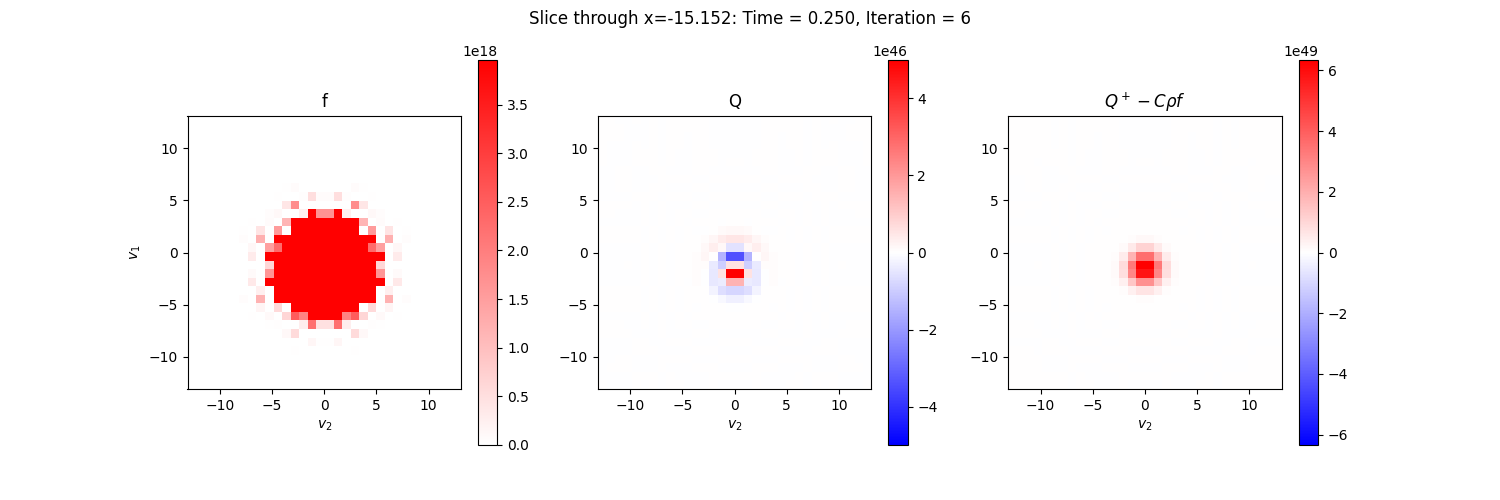
\includegraphics[width=\textwidth]{imgs/lf_output2/slice25/mat6.png}
  \end{subfigure}
  \hfill
  \begin{subfigure}[b]{\textwidth}
    \includegraphics[width=\textwidth]{imgs/lf_output2/slice50/mat6.png}
  \end{subfigure}
  \hfill
  \begin{subfigure}[b]{\textwidth}
    \includegraphics[width=\textwidth]{imgs/lf_output2/slice75/mat6.png}
  \end{subfigure}
\end{figure}

\begin{figure}[H]
  \begin{subfigure}[b]{\textwidth}
    \includegraphics[width=\textwidth]{imgs/lf_output2/slice0/mat8.png}
  \end{subfigure}
  \hfill
  \begin{subfigure}[b]{\textwidth}
    \includegraphics[width=\textwidth]{imgs/lf_output2/slice25/mat8.png}
  \end{subfigure}
  \hfill
  \begin{subfigure}[b]{\textwidth}
    \includegraphics[width=\textwidth]{imgs/lf_output2/slice50/mat8.png}
  \end{subfigure}
  \hfill
  \begin{subfigure}[b]{\textwidth}
    \includegraphics[width=\textwidth]{imgs/lf_output2/slice75/mat8.png}
  \end{subfigure}
\end{figure}

\begin{figure}[H]
  \begin{subfigure}[b]{\textwidth}
    \includegraphics[width=\textwidth]{imgs/lf_output2/slice0/mat10.png}
  \end{subfigure}
  \hfill
  \begin{subfigure}[b]{\textwidth}
    \includegraphics[width=\textwidth]{imgs/lf_output2/slice25/mat10.png}
  \end{subfigure}
  \hfill
  \begin{subfigure}[b]{\textwidth}
    \includegraphics[width=\textwidth]{imgs/lf_output2/slice50/mat10.png}
  \end{subfigure}
  \hfill
  \begin{subfigure}[b]{\textwidth}
    \includegraphics[width=\textwidth]{imgs/lf_output2/slice75/mat10.png}
  \end{subfigure}
\end{figure}
\section{Conclusions}
It is apparent that there is something weird happening with the collision operator. $Q$ and $Q^+ - C \rho f$ should give the same outputs. However, they are very distinct in all cases. I have tried looking through the code in order to determine where I am going wrong with the collision operator, but I am still unsure where the remaining issue lies. 

% I translated Jingwei's code from Python to MATLAB using ChatGPT. The code passed the built-in test so I did not think much more of the implementation. However, I am confident that the rest of the code is working. When I remove the collision operator the solution simply advects as it should. Problems only occur when I try to put the collision operator back into the equation. So, either the collision kernel code was translated improperly or I am using the algorithm incorrectly somehow. I have spent many hours trying to diagnose this issue, but unfortunately have not been able to find the cause. With more time I would go back and rederive the collision operator code myself to understand the entire algorithm.
\bibliographystyle{plain}
\bibliography{refs}
\end{document}
% \begin{figure}[H]
%   \begin{subfigure}[b]{\textwidth}
%     \includegraphics[width=\textwidth]{imgs/temp/slice0/mat0.png}
%   \end{subfigure}
%   \hfill
%   \begin{subfigure}[b]{\textwidth}
%     \includegraphics[width=\textwidth]{imgs/temp/slice25/mat0.png}
%   \end{subfigure}
%   \hfill
%   \begin{subfigure}[b]{\textwidth}
%     \includegraphics[width=\textwidth]{imgs/temp/slice50/mat0.png}
%   \end{subfigure}
%   \hfill
%   \begin{subfigure}[b]{\textwidth}
%     \includegraphics[width=\textwidth]{imgs/temp/slice75/mat0.png}
%   \end{subfigure}
%   \hfill
%   \begin{subfigure}[b]{\textwidth}
%     \includegraphics[width=\textwidth]{imgs/temp/slice100/mat0.png}
%   \end{subfigure}
% \end{figure}